% \documentclass{article}
% \usepackage[utf8]{inputenc}

% \title{ZDO 3D}
% \author{Miroslav Jirik}
% \date{May 2020}

% \begin{document}

% \maketitle

% \section{Introduction}

% \end{document}

\documentclass[xcolor=pdftex,dvipsnames,table,10pt]{beamer}
% \font\sm=csss10 scaled 1600

%\newcommand{\argmin}{\arg\!\min}
%\newcommand{\argmax}{\arg\!\max}

%-------USEFUL-PACKAGES-----------------------------------------------------------------
\usepackage{ae}
\usepackage[utf8]{inputenc} % encoding utf-8
\usepackage[czech]{babel}   % czech support
\usepackage[T1]{fontenc}    % omezí fonty na široce kompatibilní
\usepackage[all]{xy}
\usepackage{hyperref} % hypertextové odkazy
\usepackage{verbatim} % prostředí verbatim
\usepackage{epstopdf}
\usepackage{listings} % sazba zdrojových kódů, frame musí být s parametrem [fragile]
\usepackage{color}
\usepackage{amsmath}
% \usepackage{movie15}
%\usepackage{wasysym}
%\usepackage{gensymb}
\usepackage[ruled,vlined]{algorithm2e}
% \usepackage{lstlisting}


%-------CUSTOM-COLORS-------------------------------------------------------------------
\definecolor{clrfg}{RGB}{0,0,0}
\definecolor{clrfg2}{RGB}{190,215,50} % zelená: RGB: 190, 215, 50 ; HEX: #BED732
\definecolor{clrfg3}{RGB}{224,177,0} % oranžová: RGB: 224, 177, 0 ; HEX: #E0B100
\definecolor{clrbg}{RGB}{255,255,255}
%\definecolor{clrbg2}{RGB}{200,200,250}
\definecolor{clrbg3}{RGB}{224,224,225} % světle šedivá: RGB: 204, 204, 205 ; HEX: #CCCCCD
% text (tmavě šedivá): RGB: 153, 153, 153 ; HEX: #999999

%-------PRESENTATION-LAYOUT-DEFINITION--------------------------------------------------
\mode<presentation>{
	\usetheme{Dresden}
%	\usecolortheme{beaver}
	
	\setbeamercolor{alerted text}{fg = clrfg2}
	\setbeamercolor{background canvas}{bg = clrbg}
	\setbeamercolor{block title}{bg = clrfg3, fg = clrfg}
	\setbeamercolor{block body}{bg = clrbg3, fg = clrfg}
	\setbeamercolor{frametitle}{fg = clrfg}
	\setbeamercolor{item projected}{fg = clrbg}
	\setbeamercolor{sidebar}{bg = clrbg}
	\setbeamercolor{sidebar}{parent = palette primary}
	\setbeamercolor{structure}{bg = clrfg2, fg = clrfg}
	\setbeamercolor{subsection in sidebar}{fg = clrbg}
	\setbeamercolor{subsection in sidebar shaded}{fg = clrbg}
	\setbeamercolor{title}{fg = clrfg}
	\setbeamercolor{titlelike}{fg = clrbg}
	\setbeamercolor{section in head/foot}{fg = clrfg, bg = clrbg3}

	% Zobrazi (zakomentovat) nebo zmizi (odkomentovat) navigacni symboly
	\setbeamertemplate{navigation symbols}{}	

	% Zobrazi (odkomentovat) prazdnou paticku
	% \setbeamertemplate{footline}{}
	% Definuje vlastni paticku
	\setbeamertemplate{footline}{
		\hspace*{1ex}
 		{
\includegraphics[scale = 0.25, trim = 0cm 0.1cm 2.3cm 2.5cm]{./EU_logolink.png}
 		\hfill%
 		
\includegraphics[scale = 0.15, trim = 2.3cm 1.3cm 2.3cm 2.5cm]{./KKY_logo_en.pdf}} % da sedat do \logo{}, ale pak tam je zbytecne moc mista mezi logem a patickou
		\begin{beamercolorbox}[wd = \paperwidth, ht = 2.25ex, dp = 1ex,  rightskip = 3ex]{section in head/foot}
			\usebeamerfont{author in head/foot}
			\hspace*{2ex}
			\insertshorttitle
		\end{beamercolorbox}
	}

	\setbeamertemplate{headline}{
%		\leavevmode
		\begin{beamercolorbox}[wd = \paperwidth, ht = 2.25ex, dp = 3ex,  rightskip = 3ex]{section in head/foot}
%			\hbox to .5\paperwidth{\hspace{.5em}
			\vskip2pt
			\insertnavigation{7cm} 
%			\hfil
		\end{beamercolorbox}%
		}
	
	% Zobrazi (odkomentovat) prazdnou hlavicku
%	\setbeamertemplate{headline}{}
}

%-------INFORMATION---------------------------------------------------------------------
\title{Computer Vision}
\subtitle{3D}
\author{Zdenek Krnoul, Miroslav Jirik}

\institute[KKY]{Department of Cybernetics \\ Faculty of Applied Sciences \\ University of West Bohemia \newline\\ ESF projekt Západočeské univerzity v Plzni \\ reg. č. CZ.02.2.69/0.0/0.0/16\_015/0002287}
\date{} % Aby bylo na prvni strance datum vytvoreni, staci dat do slozenejch zavorek \today
%\logo{
\includegraphics[scale = 0.15, trim = 2.3cm 1.5cm 2.3cm 2.5cm]{./KKY_logo_en.pdf}} % lepsi je to definovat v paticce

%-------BEGIN-OF-DOCUMENT---------------------------------------------------------------
\begin{document}

%-------TITLE-PAGE----------------------------------------------------------------------
\begingroup 
\setbeamertemplate{headline}{}

\begin{frame}
	\titlepage
\end{frame}

%-------PAGE-NUMBERING------------------------------------------------------------------
% Nastavi pocitani stranek
\addtocounter{framenumber}{-1}
\expandafter\def\expandafter\insertshorttitle\expandafter{%
	\insertshorttitle \hfill \insertframenumber\,/\,\inserttotalframenumber
}

%-------PRESENTATION-SLIDES-------------------------------------------------------------

\begin{frame}
\frametitle{3D vidění - obsah}
\begin{itemize}
	\item Úvod do 3D vidění
    \begin{itemize}
        \item Vstupní data a principy snímání
    \end{itemize}
    \item rep
    \begin{itemize}
    \item nalezení a klasifikace objektů ve scéně, často také určení polohy, orientace, měřítka apod.
    \end{itemize}
\end{itemize}
\textit{Pozn. V praktických úlohách se často snažíme vyhnout 3D vidění, převést úlohu na 2D. Důvodem jsou požadavky na robustnost, nízkou cenu a velkou efektivitu využití systémů počítačového vidění.}
\end{frame}

\begin{frame}
\frametitle{3D vidění - základní typy úloh:}
\begin{itemize}
	\item Rekonstrukce
    \begin{itemize}
    \item nalezení  geometrických  a  fyzikálních  parametrů  objektů  ve  3D scéně  tak,  aby  bylo  možno rekonstruovat jejich 3D tvar
    \end{itemize}
    \item Rozpoznávání
    \begin{itemize}
    \item nalezení a klasifikace objektů ve scéně, často také určení polohy, orientace, měřítka apod.
    \end{itemize}
\end{itemize}
\textit{Pozn. V praktických úlohách se často snažíme vyhnout 3D vidění, převést úlohu na 2D. Důvodem jsou požadavky na robustnost, nízkou cenu a velkou efektivitu využití systémů počítačového vidění.}
\end{frame}

\begin{frame}
\frametitle{Vstupní data, možnosti snímání}
\begin{itemize}
	\item intenzitní obraz(y) - (RGB) (často je potřeba více pohledů na scénu z různých úhlů)
	\item stereovidění – právě dva intenzitní obrazy, kalibrované kamery
	\item hloubkové senzory - jsou v dnešní době běžný postup 
\end{itemize}

    \begin{figure}[!ht]
	\centering
	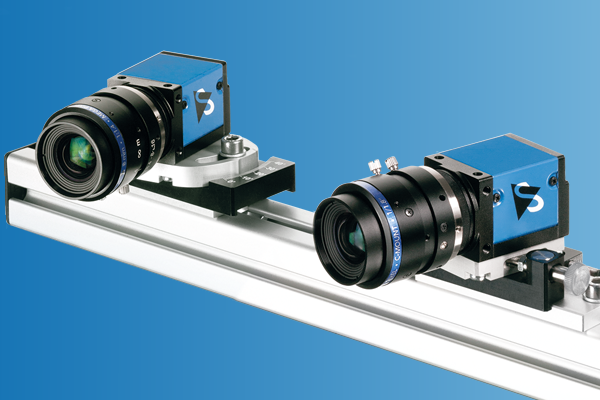
\includegraphics[width = 0.3\textwidth]{./stereo}
	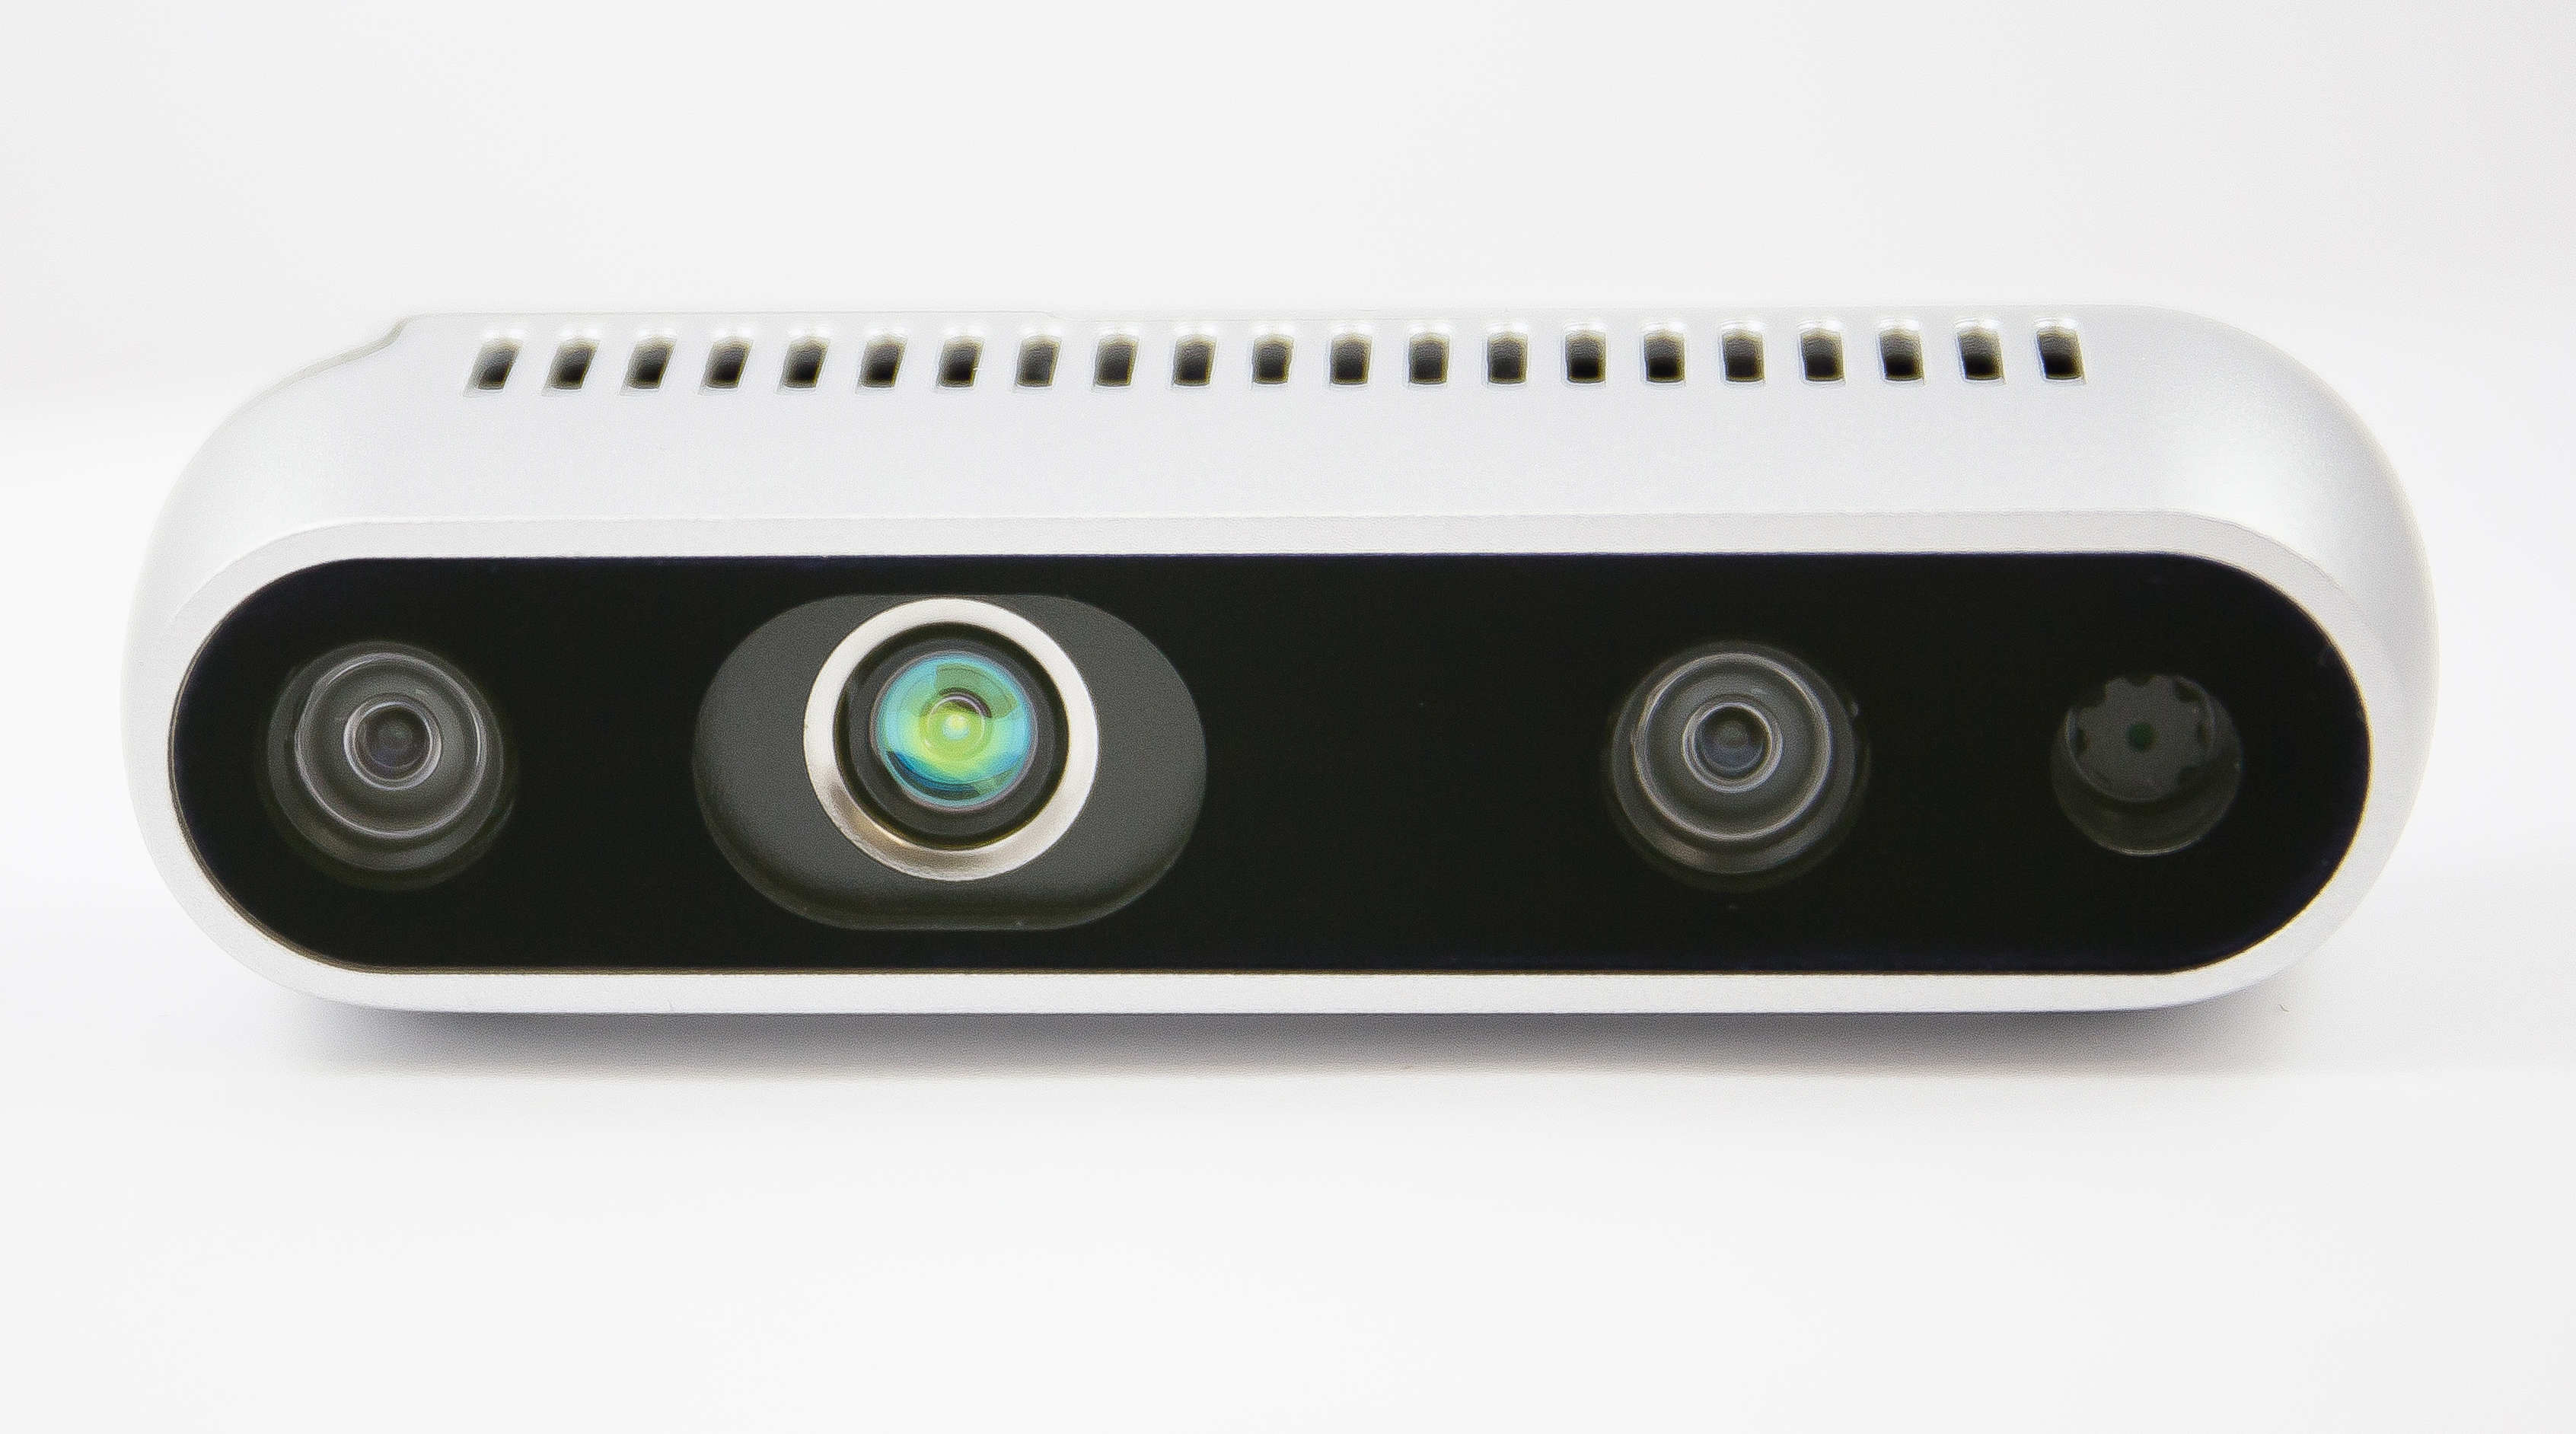
\includegraphics[width = 0.3\textwidth]{./intel}
	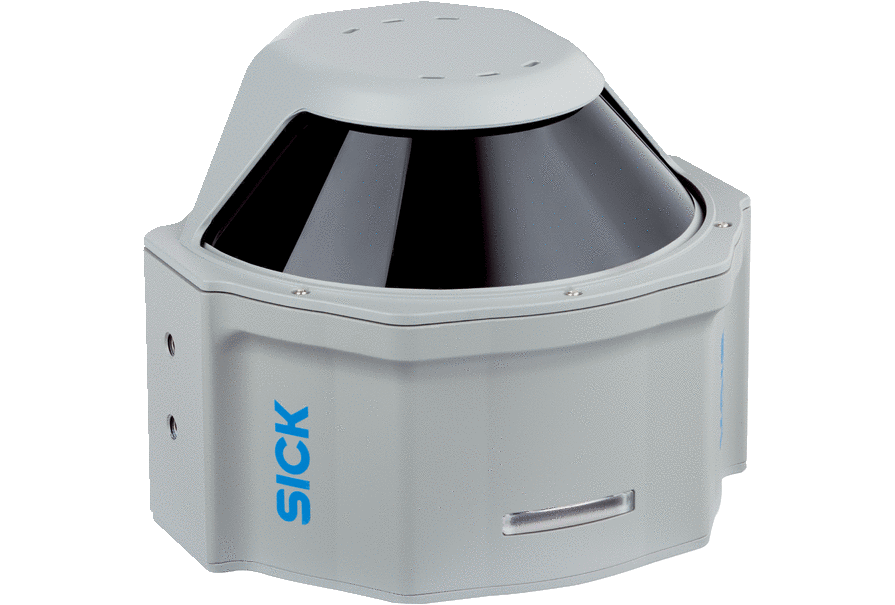
\includegraphics[width = 0.3\textwidth]{./lidar}
	\end{figure}
	
\end{frame}

\begin{frame}
\frametitle{Hloubková mapa}
\begin{enumerate}
	\item Často používáme specializovaný senzor či kameru např. dobře známé MS Kinect, Intel RealSense aj. 
	\item Nebo technikou zaostřování objektivu
	\item Nebo výpočtem pouze z intenzitních obrazů, např. zmíněné stereovidění - tzv. husté stereo
	\item A další techniky založené např. na odrazu světla, známé textuře aj.
\end{enumerate}
	\begin{figure}[!ht]
	\centering
	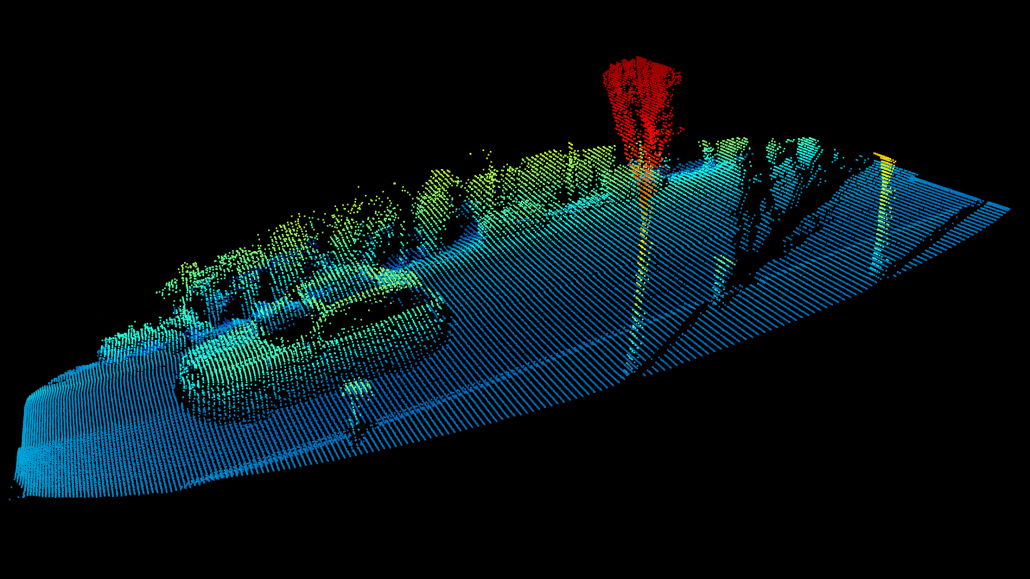
\includegraphics[width = 0.45\textwidth]{./lidar-car}
	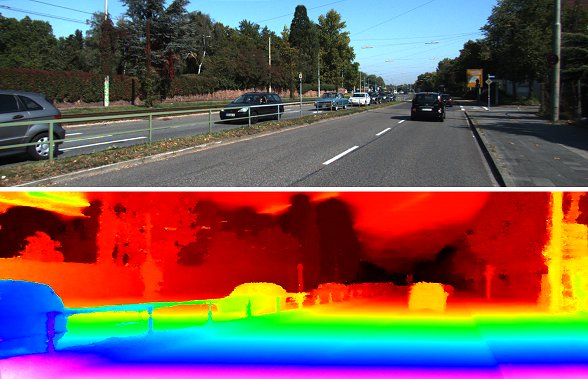
\includegraphics[width = 0.5\textwidth]{./kitti}
	\caption{Blickfeld, KITTI dataset}
	\end{figure}
\end{frame}

\begin{frame}
% \frametitle{Hloubková mapa - senzory:}
Hloubkové senzory:
\begin{itemize}
\item Strukturované osvětlení – scéna osvětlena pomocný zdrojem světla
\item Laserové - podobný princip jako radary a sonary 

	\begin{figure}[!ht]
	\centering
	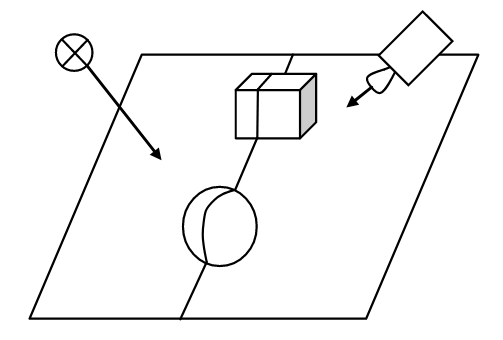
\includegraphics[width = 0.3\textwidth]{./prouzek}
	\caption{Společný princip zařízeních při získávání hloubkové mapy.}
	\end{figure}
% 	\includemovie{1cm}{1cm}{ani.gif}

\end{itemize}
\end{frame}

\begin{frame}
Princip strukturovaného osvětlení:
\begin{itemize}
\item Scéna/povrch osvětlen např. úzkým proužkem světla nebo jedinečným vzorem (MS Kinect I - infrared) a scéna snímána z jiného úhlu,  (problém stínů)
\item Nutná kalibrace projektoru a kamery (často zabudováno pevně v přístroji)
\item Nutný algoritmus pro dekódování promítnutého vzoru
\item Dále už jen princip stereovidění, viz níže
\item Dobrá přesnost je získána pro jednobarevné nelesklé povrchy, u Kinectu ruší jiné IR záření (např. slunce)
\end{itemize}
    \begin{figure}[!ht]
	\centering
	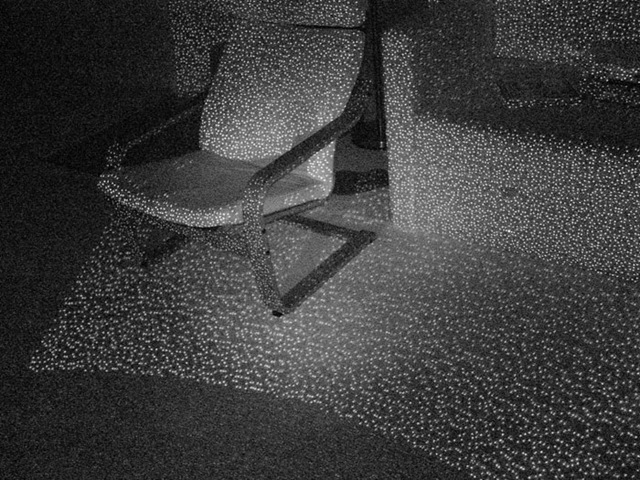
\includegraphics[width = 1.0\textwidth]{./kinect1}
	\end{figure}
\end{frame}

\begin{frame}

\begin{itemize}
\item Strukturovaného osvětlení: Moiré  proužky:
    \begin{itemize}
    \item Obvykle promítnuty tři nebo čtyři fázově posunuté sinusové vzory na povrch 
    \item Snímky deformovaných obrazců zachycené kamerou se používají k výpočtu fázové mapy, která obsahuje informace o výšce povrchu
    \item Vysoká přesnost je získána pro jednobarevné nelesklé povrchy
    \end{itemize}
\end{itemize}
	\begin{figure}[!ht]
	\centering
	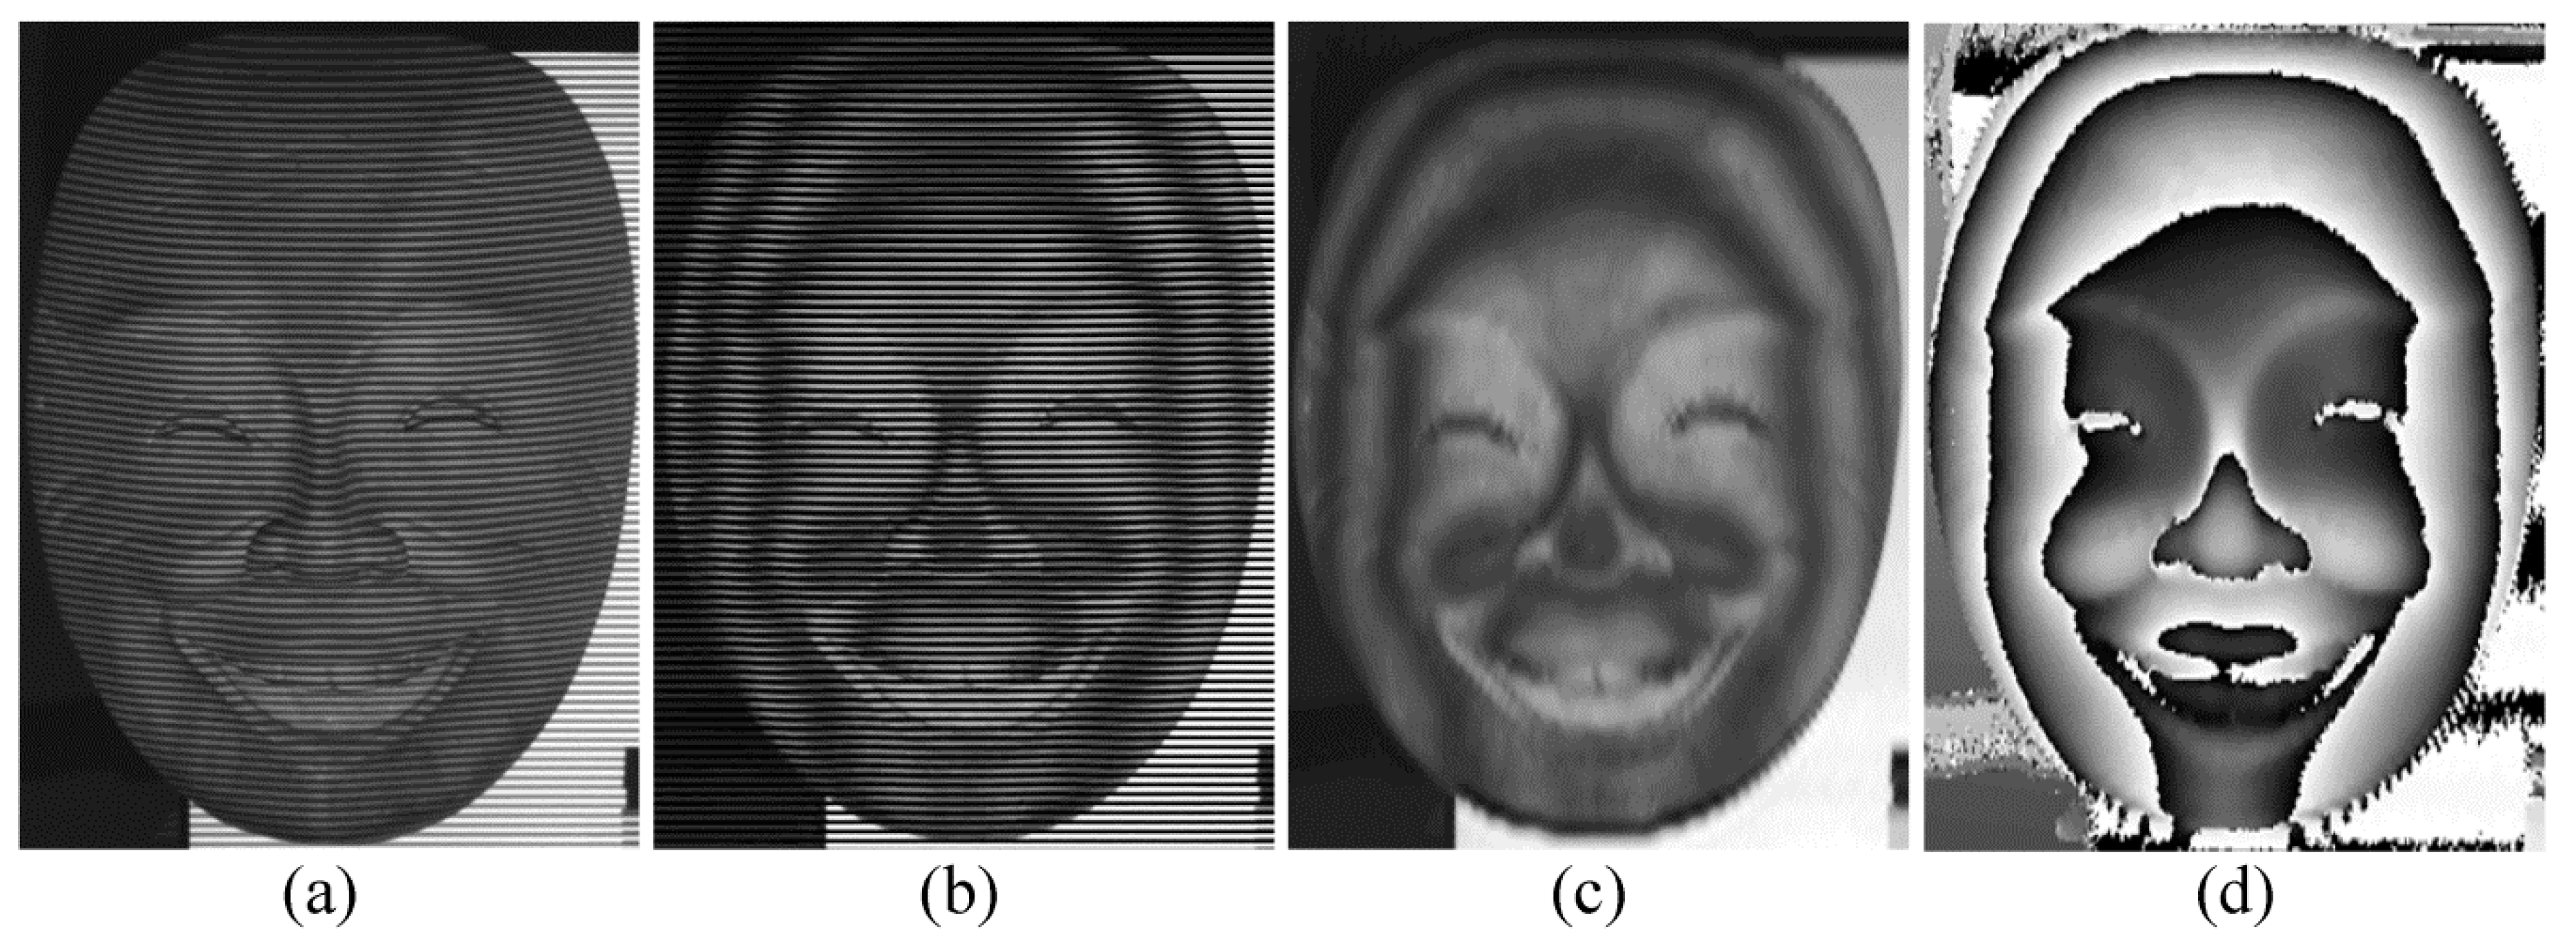
\includegraphics[width = 1.0\textwidth]{./moire}
	\end{figure}
Pozn. Na podobném principu existuje mnoho dalších metod 
\end{frame}

\begin{frame}
Princip laserového měření:
\begin{itemize}
\item Měří fázový posun mezi vyslaným a přijatým signálem (např. bodově - lidar, nebo jako obraz - ToF kamera - MS Kinect II)
\end{itemize}
	\begin{figure}[!ht]
	\centering
	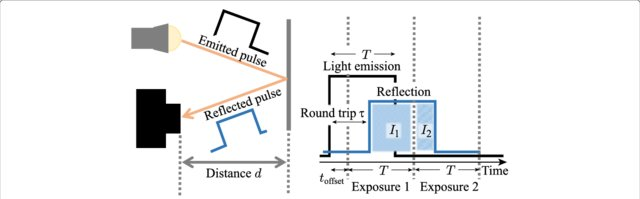
\includegraphics[trim=30 0 30 0,clip, width = 1.0\textwidth]{./tof}
	\caption{Převzato z \cite{Kitano2017}}
	\end{figure}
% 	\includemovie{1cm}{1cm}{ani.gif}
\end{frame}


% princip  Moiré  proužků –scéna je osvětlena přes pravidelnou mřížku zrovnoběžných proužků. Podle jejich šířky lze určovat sklon povrch.Princip proměnného zaostření objektivu–po detekci maximální ostrosti je vzdálenost odečtena znastavení zaostření objektivu


\begin{frame}
Princip proměnného zaostření objektivu:
\begin{itemize}
\item 
\end{itemize}
	\begin{figure}[!ht]
	\centering
	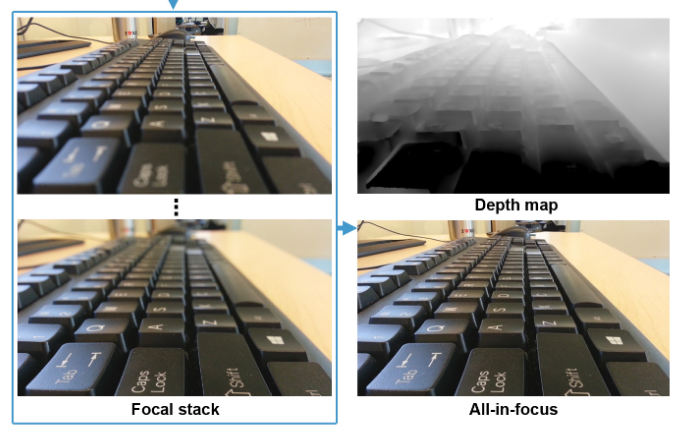
\includegraphics[width = 0.8\textwidth]{./fokus}
	\caption{Pro mobilní telefon, převzato z \cite{Suwajanakorn_2015_CVPR}}
	\end{figure}
\end{frame}

 
\begin{frame}
% \frametitle{3D vidění - Perspektivní kamera}
Princip stereovidění:
\begin{itemize}
\item Využívá obecný \textbf{model perspektivní kamery} - popis projekce $ 3D $ prostoru do $ 2D $ prostoru (obrazová rovina)
\item Vždy se jedná o \textbf{středovou projekci}
\end{itemize}

\begin{figure}[h]
\centering
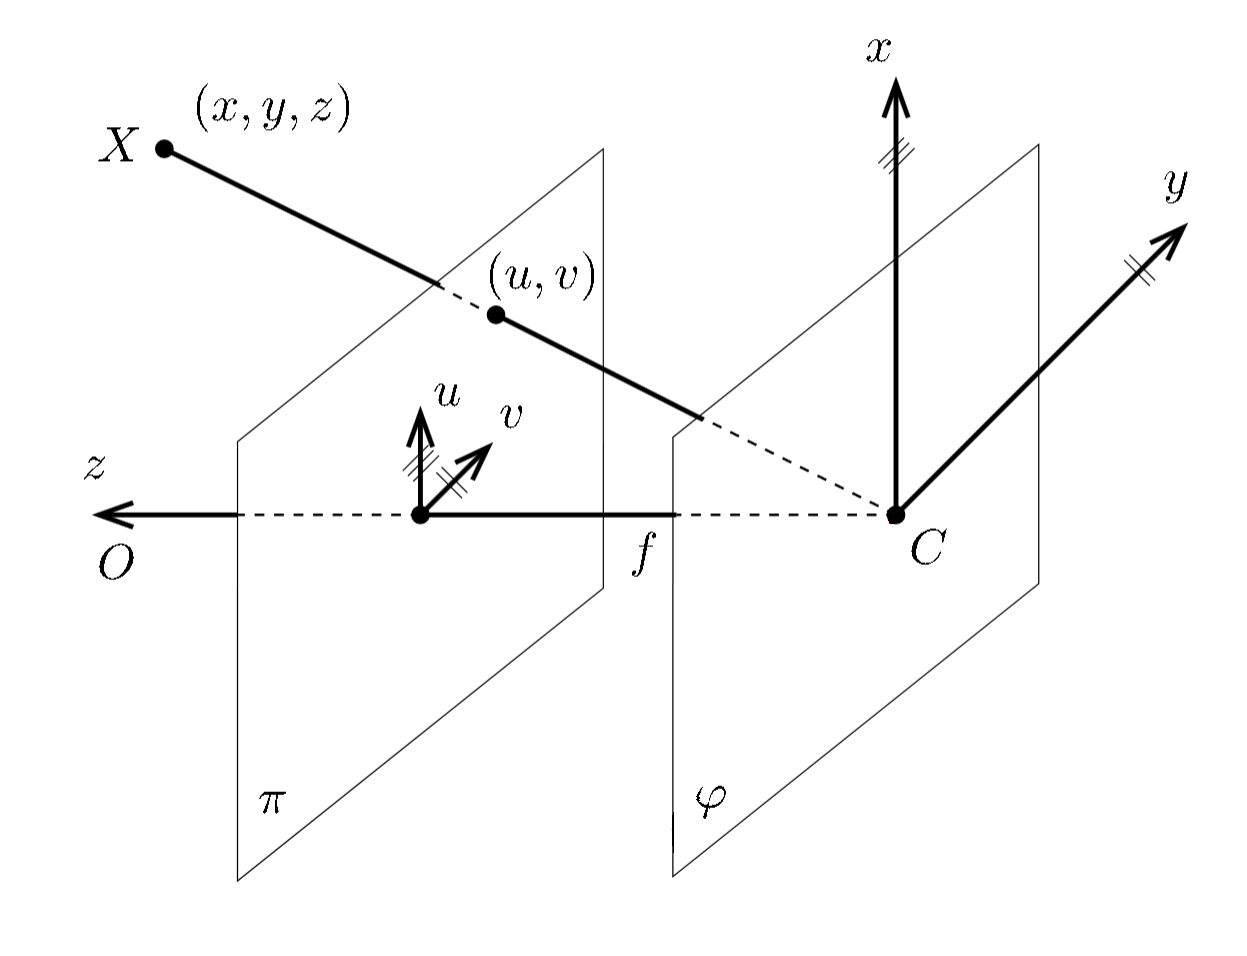
\includegraphics[width=0.65\textwidth]{./fig01}
\end{figure}
\textit{
Pozn.  speciální případ ... střed projekce leží v nekonečnu $ \rightarrow $ \textbf{afinní kamera} a jde o zobecnění tzv. paralelní projekce}
\end{frame}

\begin{frame}
\begin{figure}[h]
\centering
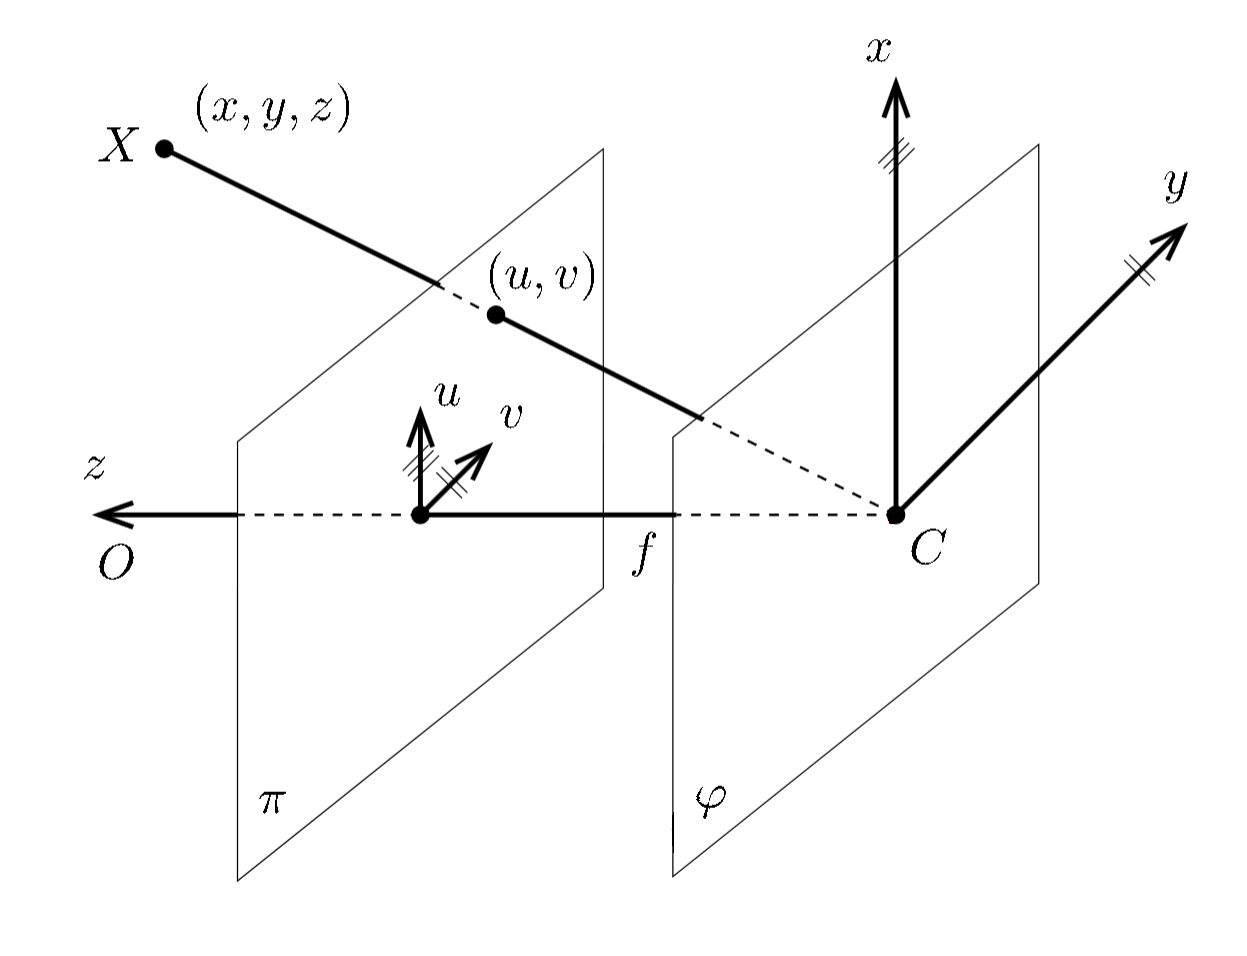
\includegraphics[width=0.55\textwidth]{./fig01}
\end{figure}

\begin{itemize}
\item Perspektivnı kamera má 11 stupňů volnosti: 1x ohnisková
vzdálenost v pixelech + 1x poměr stran pixelu + 1x zkosenı os
+ 2x počátek obrázku + 3x posun + 3x rotace kamery = 11
DOFs (degree of freedom)
\item Pro určení použijeme algoritmus kalibrace kamery (problém je lineární v homogenních souřadnicích)
\item Teoreticky stačí 5,5 prostorových bodů
\end{itemize}

\end{frame}

\begin{frame}

\begin{figure}[h]
 \centering
 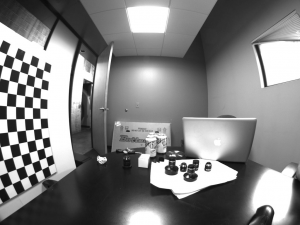
\includegraphics[width=0.45\textwidth]{./fig17}
 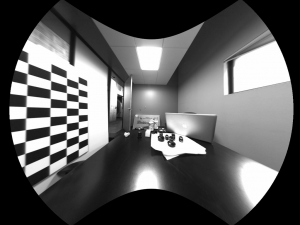
\includegraphics[width=0.45\textwidth]{./fig16}
 \end{figure}
\begin{itemize}

\item Někdy je nutné provést korekci zkreslení souřadnic obrázku - tzv. radialní zkreslení
\item Efekt je způsoben nedokonalostí středového promítání, které je fyzicky provedeno přes čočku(y) objektivu
\end{itemize}
\end{frame}

\begin{frame}

\begin{itemize}
\item U stereovidění máme dva pohledy na stejnou scénu z různých směrů
\begin{itemize}
\item Pohledy mohou být získány souběžně v jeden okamžik (např. dvě kamery)
\item Pohyb přístroje před objektem (např. obcházím kolem sochy a fotím ji z různých úhlů)
\item Pohyb objektu před přístrojem (např. otáčím jablkem před kamerou)
\end{itemize}
\item Tyto úlohy jsou duální a vedou na stejné řešení
\end{itemize}
\begin{figure}[h]
\centering
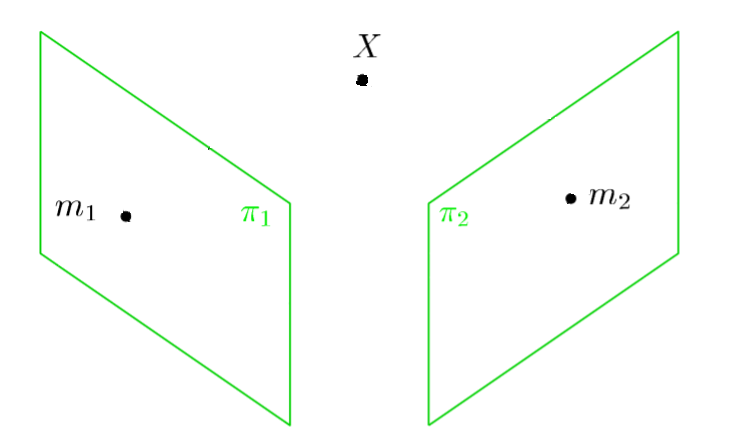
\includegraphics[width=0.7\textwidth]{./epi1c}
\label{fig:epi1}
\end{figure}

\end{frame}

\begin{frame}
Stereovidění - 3D rekonstrukce

\begin{figure}[h]
\centering
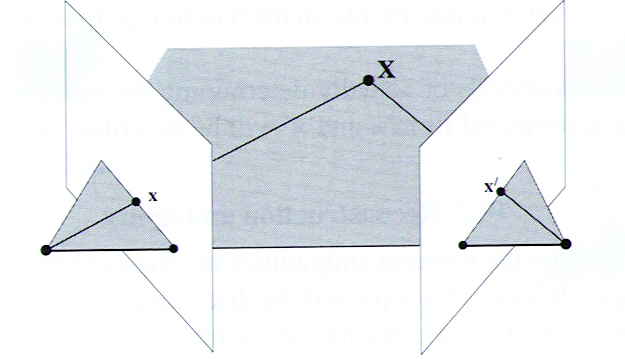
\includegraphics[width=0.7\textwidth]{./epi3}
\label{fig:epi3}
\end{figure}
\begin{itemize}
\item Pokud známe obě kamery zkalibrované
\item A současně máme korespondující pár
\item Pak můžeme určit 3D souřadnici neznámého bodu
\end{itemize}
\end{frame}


\begin{frame}
\frametitle{Teorie 3D vidění (Marrova teorie)}
4 úrovně reprezentace 3D scény:
\begin{itemize}
	\item intenzitní obraz
	\item prvotní  náčrtek
	\item 2 1/2 dimenzionální náčrtek
    \item plná 3D reprezentace	
\end{itemize}
	\begin{figure}[!ht]
	\centering
	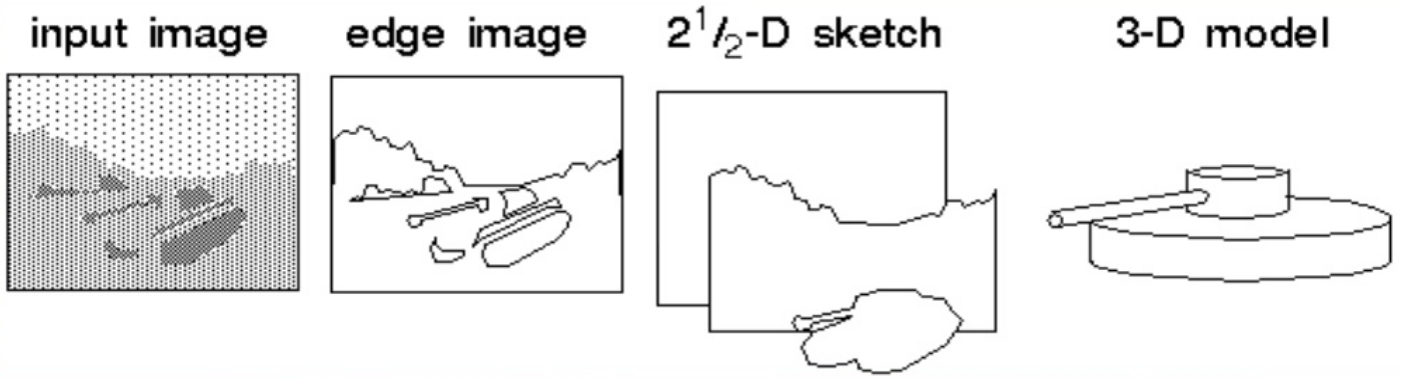
\includegraphics[width = 1.0\textwidth]{./tank}
	\end{figure}
\end{frame}

\begin{frame}
Prvotní náčrtek:
	\begin{figure}[!ht]
	\centering
	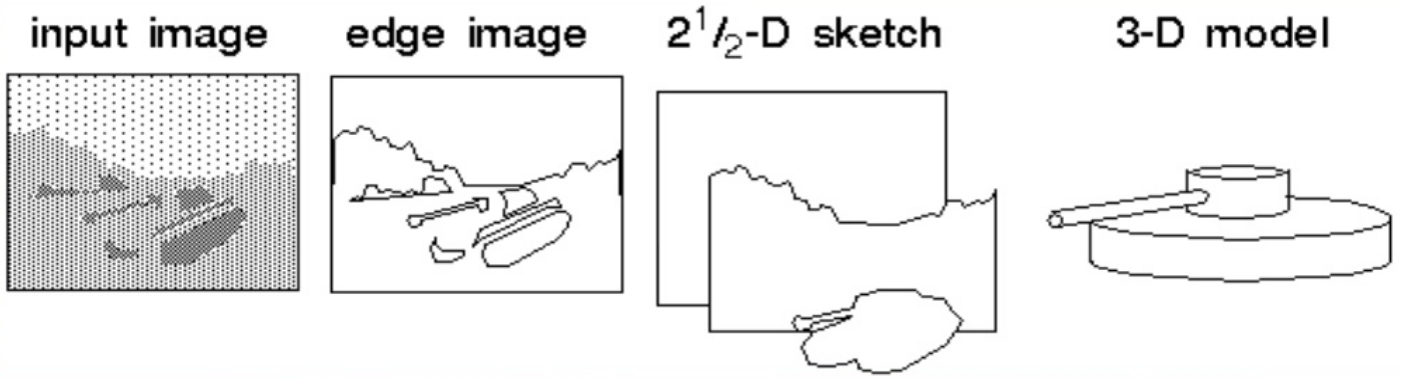
\includegraphics[trim=250 0 650 70,clip, width = 0.4\textwidth]{./tank}
	\end{figure}
\begin{itemize}
	\item Obsahuje informace o velikostech a směrech významných jasových změn v obraze 
	\item Jejich  vzájemné  geometrickém  uspořádání
	\item Předpokládáme,  že  takto  získané  čáry  a  skvrny zachovávají informaci potřebnou pro pozdější 3D reprezentaci
\end{itemize}
\end{frame}

\begin{frame}
2 1/2 rozměrný náčrtek:
	\begin{figure}[!ht]
	\centering
	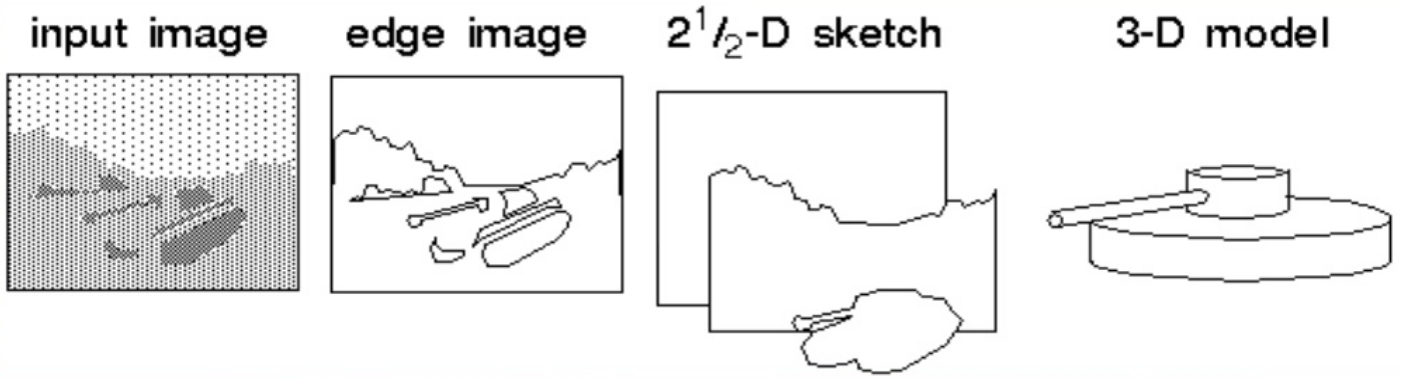
\includegraphics[trim=600 0 300 80,clip, width = 0.4\textwidth]{./tank}
	\end{figure}
\begin{itemize}
	\item Pro jeho získání se používá informace obsažená v prvotním náčrtku
	\item Používají se různé techniky, souhrnně nazývané „tvar  z X“ 
	\begin{itemize}
	    \item Tvar ze stereovidění
	    \item Tvar z pohybu (optický tok)
	    \item Tvar z jasu
	    \item Tvar z textury
	\end{itemize}
\end{itemize}
\end{frame}

\begin{frame}
Plná 3D reprezentace objektu:
	\begin{figure}[!ht]
	\centering
	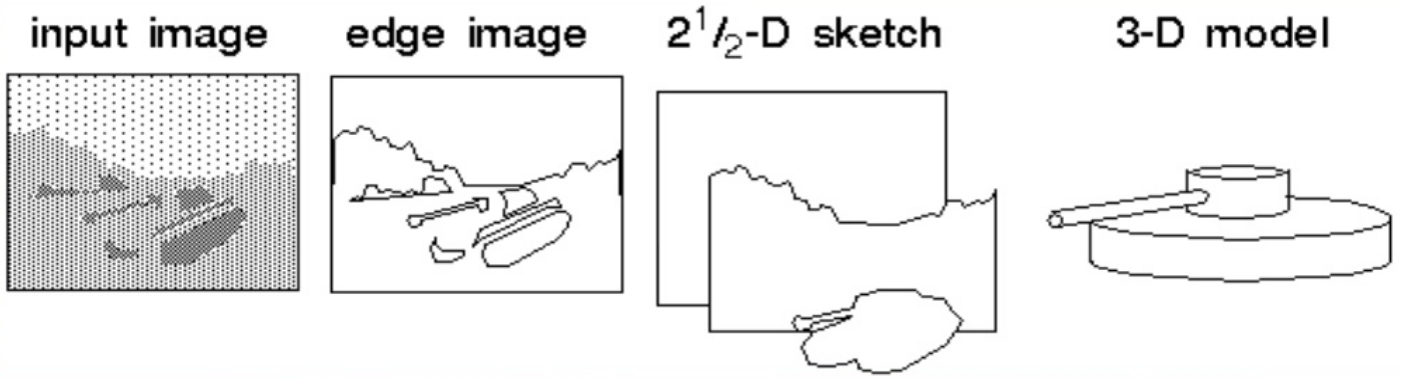
\includegraphics[trim=950 0 0 80,clip, width = 0.4\textwidth]{./tank}
	\end{figure}
\begin{itemize}
	\item Opírá se o  geometrické  vlastnosti,  které  lze  v obraze  nalézt
	\item Geometrické  vlastnosti jsou vyjádřené  vzhledem k souřadnému systému vycházejícímu z tvaru objektu
	\item Základní geometrické vlastnosti:
	\begin{itemize}
	    \item střed (nejčastěji těžiště)
	    \item celková velikost 
	    \item zobecněná osa symetrie (pokud je)
	\end{itemize}
\end{itemize}
\end{frame}

\begin{frame}
\frametitle{Modely 3D objektů}
Lze rozdělit na:
\begin{itemize}
	\item deskriptivní – plně popisují tvar objektu, definována odrazivost a osvětlení, z takového modelu lze vytvořit syntetický intenzitní obraz i syntetickou hloubkovou mapu pro libovolné místo pozorování
	\item diskriminační – slouží k odlišení objektů několika tříd
\end{itemize}

Používané typy reprezentace:
\begin{itemize}
	\item drátový model - graf,jehož  vrcholy  odpovídají  3D  bodům  (často  vrcholům  objektu),  hrany  odpovídají  hranicím (nespojitostem normál k povrchu). Nehodí se pro popis objektů s křivočarými povrchy
\end{itemize}

\end{frame}

\begin{frame}
\begin{itemize}
	\item CSG (constructive solid geometry) model - používá  jako  základ  množinu  jednoduchých  3D  objektů,  jako  hranoly,  kužely,  válce,  koule,  krychle, kvádry  ap.  a  kombinuje  je  v  určité  pozici,  zvětšení  a  orientaci  pomocí  jednoduchých  množinových operací,  jako  průnik,  sjednocení,  rozdíl,  ap.  Model  je  reprezentován  stromem;  listy  odpovídají jednotlivým  elementárním  tělesům,  vyšší  uzly  představují  množinové  operace.  Toto  vyjádření  je výpočetně velmi náročné.
	\begin{figure}[!ht]
	\centering
	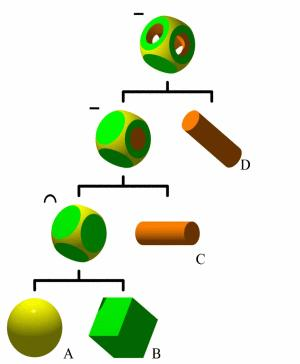
\includegraphics[width = 0.3\textwidth]{./csgtree}
	\end{figure}
\end{itemize}
\end{frame}

\begin{frame}
GEON (z angl. geometrical ions)
\begin{itemize}
	\item  Zdůrazňuje  kvalitativní  charakter  reprezentace  objektů
	\item  3D objekty  jsou  složeny  z několika  sousedících GEONů
	\item Navrženo 36 základních GEONů
	\item Každý GEON je charakterizován čtveřicí kvalitativních vlastností:
	    \begin{itemize}
	    \item hranice – rovná / křivá 
	    \item symetrie – středová / osová / žádná 
	    \item změna velikosti – stálá / zvětšující se / zvětšující i zmenšující se 
	    \item osa – přímá / křivá
	    \end{itemize}
	\begin{figure}[!ht]
	\centering
	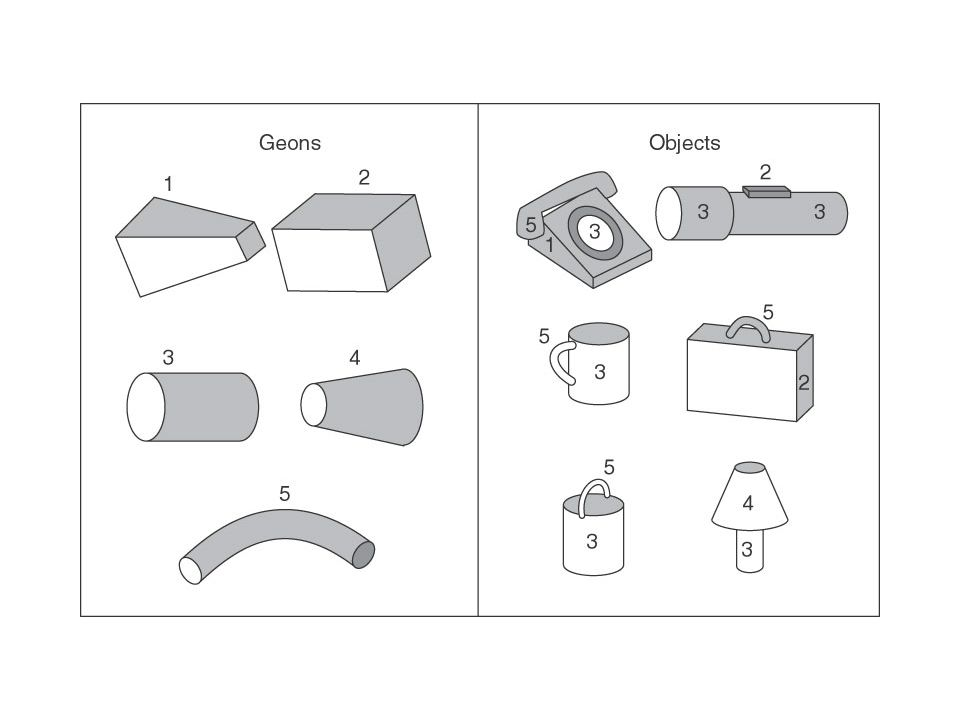
\includegraphics[width = 0.6\textwidth]{./geons}
	\end{figure}
\end{itemize}
\end{frame}




% Ostatni strany prezentace

\section{Object representation}
\begin{frame}{Object representation}
\begin{itemize}
    \item Volumetric
    \item Surface
    \begin{itemize}
        \item Triangulated mesh
        \item Nurbs
    \end{itemize}
\end{itemize}

\end{frame}

\begin{frame}[t,allowframebreaks]{3D Vision}
    \tableofcontents
    
\end{frame}

\begin{frame}{Object representation}
\begin{itemize}
    \item Geometry
    \item Topology
\end{itemize}
\end{frame}

\subsection{Geometry and Topology}
\begin{frame}{Geometry and Topology}
    \begin{columns}
        \column{0.6\textwidth}
            \begin{block}{Geometry}
            Geometry 
            % (from the Ancient Greek: γεωμετρία; geo- "earth", -metron "measurement") 
            is a branch of mathematics concerned with questions of shape, size, relative position of figures, and the properties of space \cite{de2015mathematizing}. A mathematician who works in the field of geometry is called a geometer.
            \end{block}
            \begin{block}{Topology}
            In mathematics, topology 
            % (from the Greek τόπος, 'place', and λόγος, 'study')
            is concerned with the properties of a geometric object that are preserved under continuous deformations, such as stretching, twisting, crumpling and bending, but not tearing or gluing.
            \end{block}
        \column{0.4\textwidth}
            \begin{figure}
                \centering
                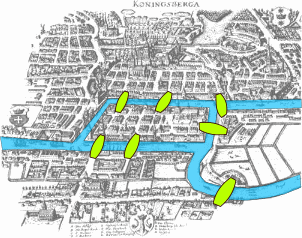
\includegraphics[width=\textwidth]{figs/Konigsberg_bridges.png}
                \caption{Seven Bridges of Königsberg 
                    \cite{euler1953leonhard, euler1741solutio,wiki:7bridges}
                }
            \end{figure}
    \end{columns}
    
    
\end{frame}


\begin{frame}[fragile]{OBJ file format}
    \begin{columns}
        \column{0.6\textwidth}
        Content of \verb+example.obj+ can be displayed with ParaView application.
            \begin{lstlisting}
            v 0.0 0.0 0.1
            v 0.0 0.1 1.0
            v 0.0 1.0 0.1
            v 0.0 1.0 1.0
            v 0.2 2.0 0.5
            
            g cellobject
            f 1 2 4 3
            f 3 4 5
            \end{lstlisting}
        \column{0.4\textwidth}
            \begin{figure}
                \centering
                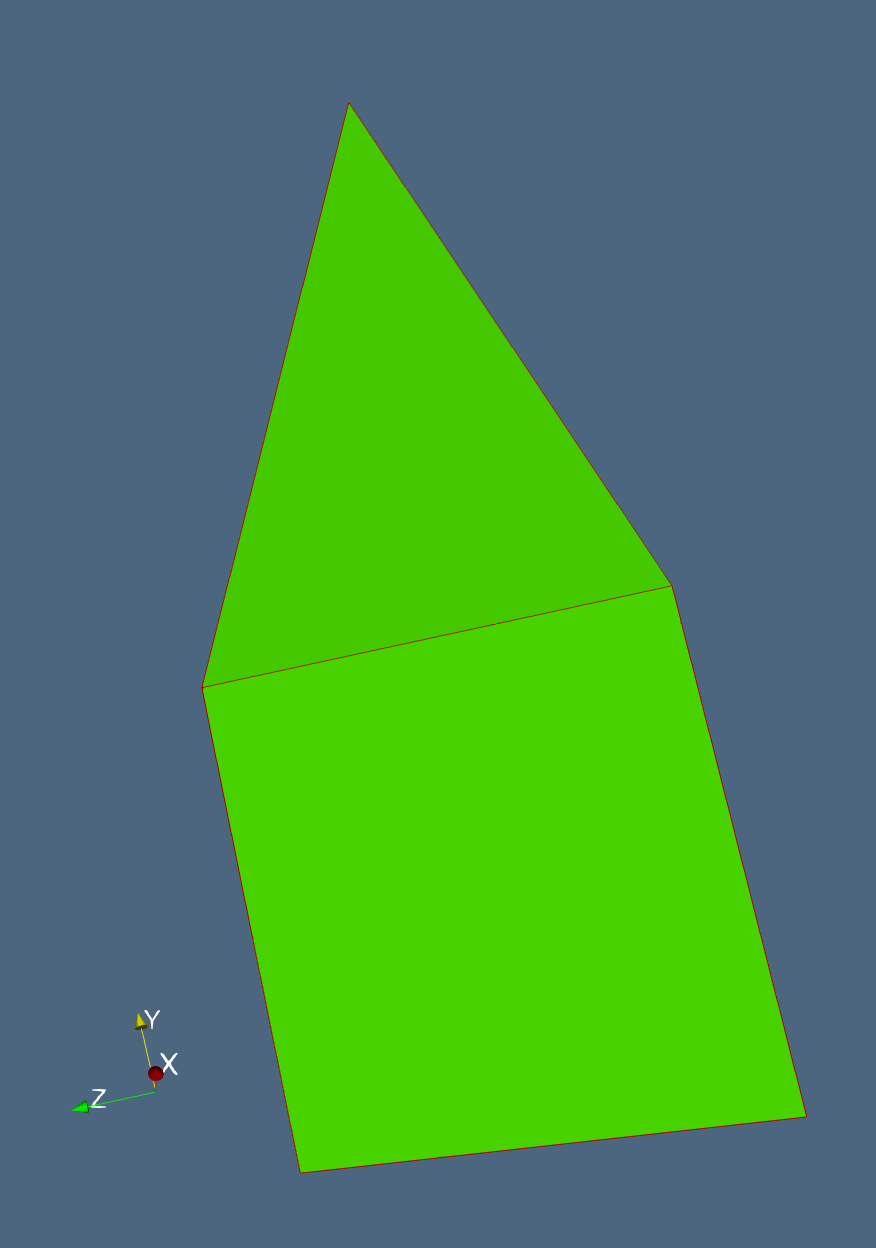
\includegraphics[width=\textwidth]{figs/example_obj.png}
                % \caption{Caption}
                % \label{fig:my_label}
            \end{figure}
    \end{columns}
\end{frame}

\begin{frame}
\vfill
\centering

\begin{beamercolorbox}[sep=8pt,center,shadow=true,rounded=true]{title}
Linear Algebraic Representation
\end{beamercolorbox}
Alberto Paoluzzi, Antonio DiCarlo \cite{DiCarlo2014}
\vfill
    
\end{frame}

\begin{frame}
\begin{figure}
    \centering
    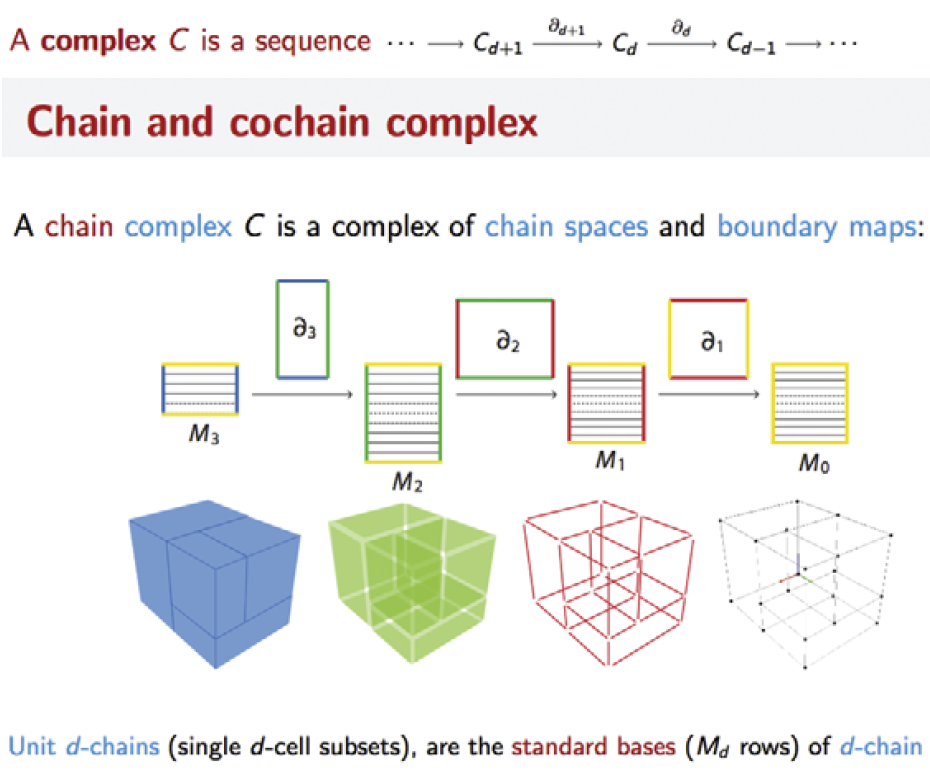
\includegraphics[width=0.95\textwidth]{figs/L02-chain-complex.png}
    % \caption{Caption}
    % \label{fig:my_label}
\end{figure}
    
\end{frame}

\begin{frame}
\begin{figure}
    \centering
    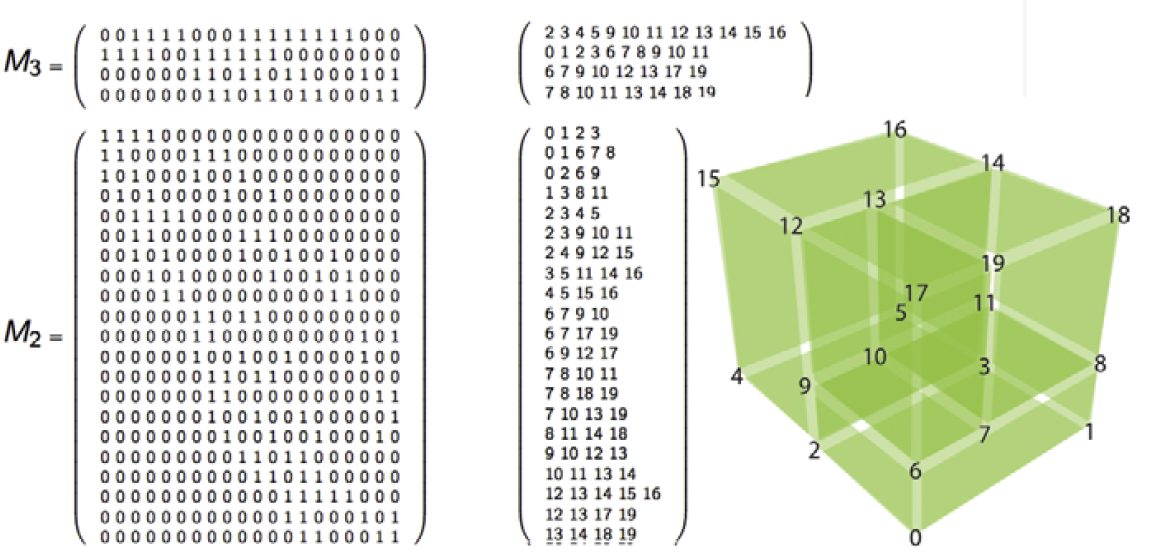
\includegraphics[width=\textwidth]{figs/L02-characteristic-matrices.png}
    % \caption{Caption}
    % \label{fig:my_label}
\end{figure}
    
\end{frame}

\begin{frame}{Point cloud}
\begin{figure}
    \centering
    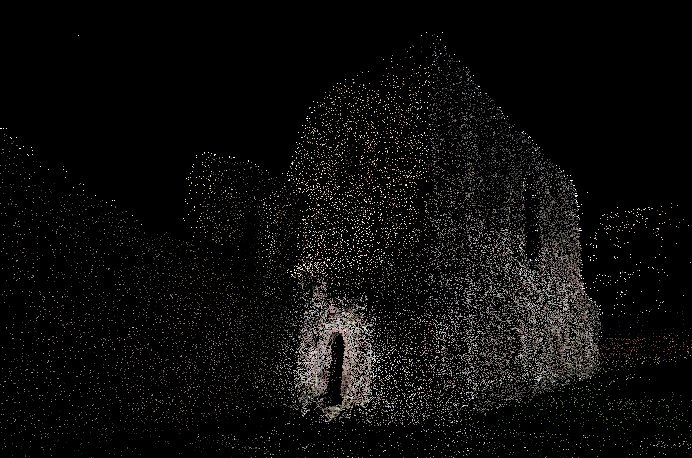
\includegraphics[width=\textwidth]{figs/Monmouth_castle_point_cloud,_created_with_Photosynth_01.jpg}
    \caption{Monmouth castle point cloud, created with Photosynth, \url{https://commons.wikimedia.org/wiki/File:Monmouth_castle_point_cloud,_created_with_Photosynth_01.jpg}}
    \label{fig:my_label}
\end{figure}
    
\end{frame}


\subsection{Triangulation}
\subsection{Delaunay triangulation}
\begin{frame}{Triangulation (terrain map)}
\begin{figure}
    \centering
    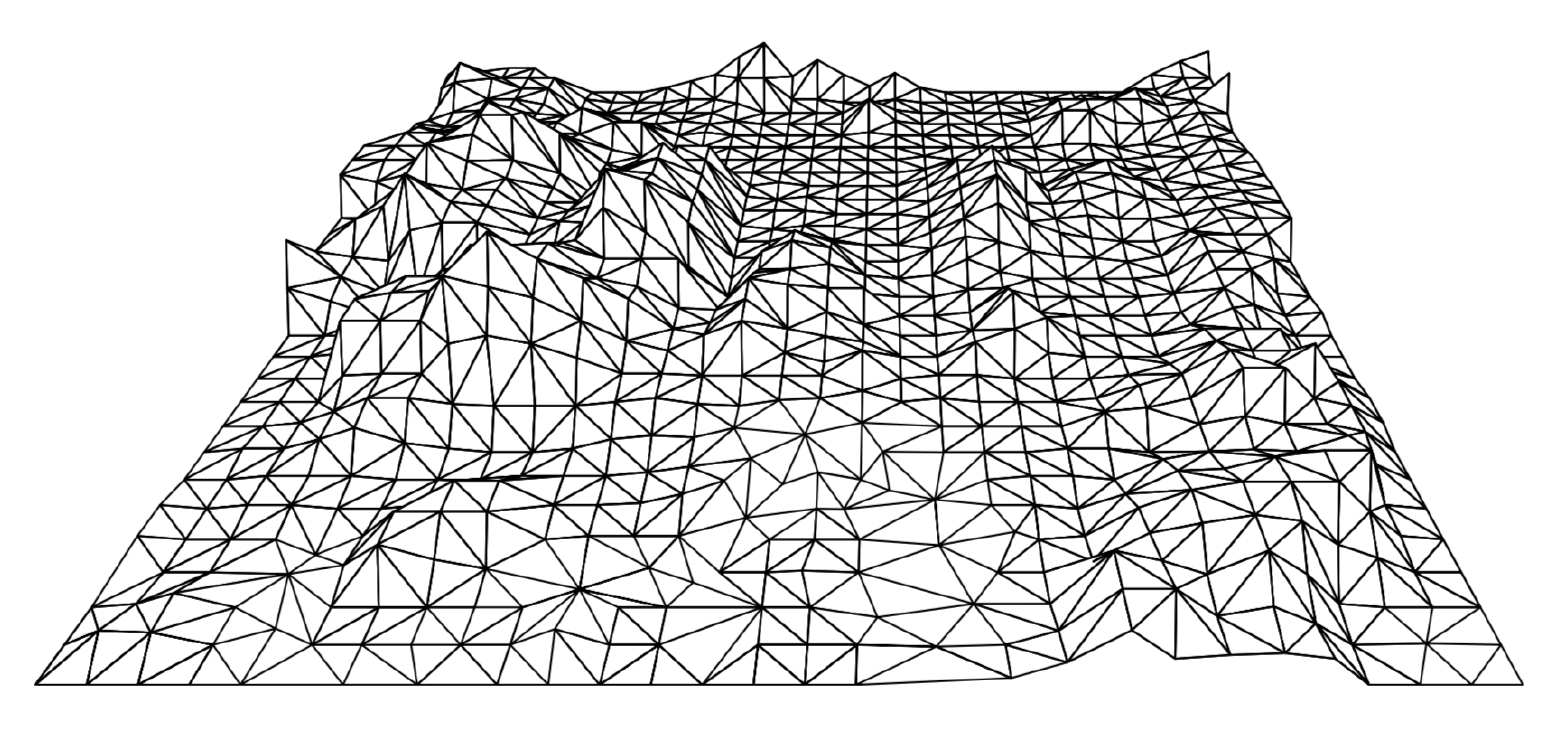
\includegraphics[width=0.9\textwidth]{figs/L07-terrain-map.png}
    % \caption{Caption}
    % \label{fig:terrain-map}
\end{figure}

\end{frame}



\begin{frame}{Triangulation}

    \begin{columns}
    	\column{.6\textwidth}
    % 	\begin{block}{}
    We first determine a triangulation of P: a
    planar subdivision whose bounded faces are
    triangles and whose vertices are the points of
    P. We then lift each sample point to its height,
    mapping every triangle in the triangulation to
    a triangle in 3-space.
    
    We get is a polyhedral terrain, the graph of a
    piecewise linear continuous function
    The polyhedral terrain as an approximation of
    the original terrain.    
    % 	\end{block}
    	\column{.4\textwidth}
    % 	\begin{block}{Generative}
    	\begin{figure}
    	    \centering
    	    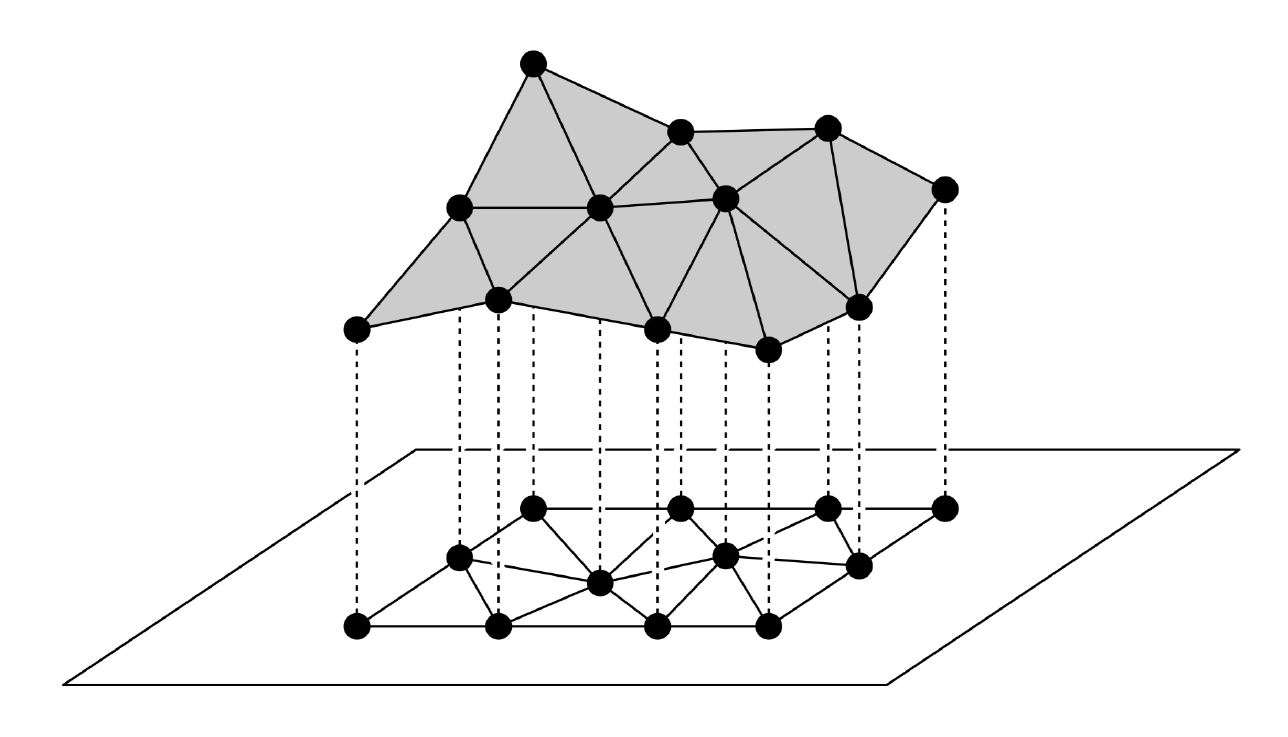
\includegraphics[width=\textwidth]{figs/L07-terrain-map-2.png}
    	   % \caption{Caption}
    	   % \label{fig:my_label}
    	\end{figure}
    % 	\end{block}
    \end{columns}

\end{frame}


\begin{frame}{Triangulations of Planar Point Sets \cite{DeBerg2008}}

    Let $P := \left\{p_1, p_2,..., p_n\right\}$ be a set of points in the plane. To be able to formally
    define a triangulation of P, we first define a maximal planar subdivision as
    a subdivision S such that no edge connecting two vertices can be added to
    S without destroying its planarity. In other words, any edge that is not in S
    intersects one of the existing edges. A triangulation of P is now defined as a
    maximal planar subdivision whose vertex set is P.
    \begin{columns}
        \column{0.6\textwidth}
     Let P be a set of n points in the plane, not all collinear, and let k
denote the number of points in P that lie on the boundary of the convex hull
of P. Then any triangulation of P has $2n - 2 - k$ triangles and $3n-3-k$ edges.
        \column{0.3\textwidth}
        \begin{figure}
            \centering
            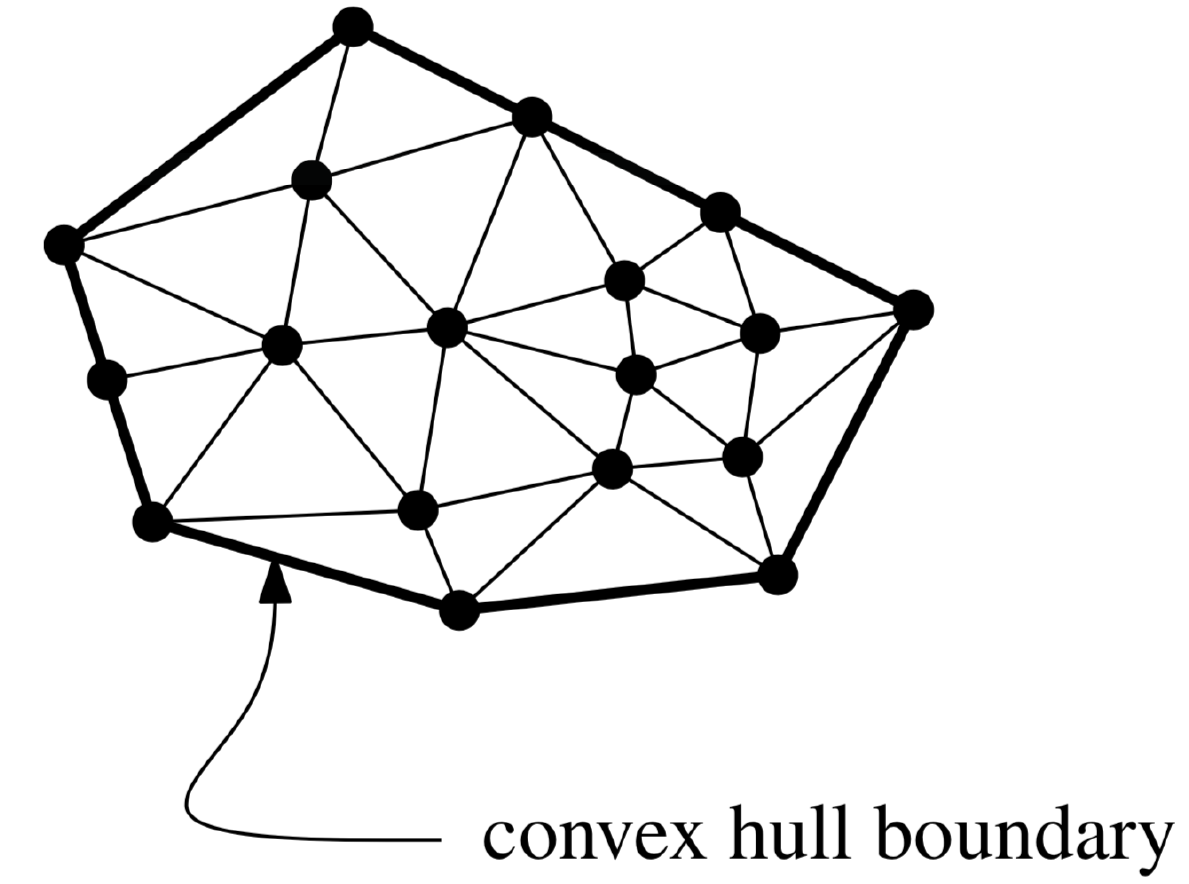
\includegraphics[width=\textwidth]{figs/L07-convex-hull.png}
            % \caption{Caption}
            % \label{fig:my_label}
        \end{figure}
    \end{columns}
\end{frame}


\begin{frame}{The Delaunay Triangulation}
    \begin{columns}
        \column{0.6\textwidth}
        Delaunay triangulation for a set P of discrete
points in a plane is a triangulation DT(P)
such that no point in P is inside the
circumcircle of any triangle in DT(P).

Delaunay triangulations maximize the
minimum angle of all the angles of the
triangles in the triangulation.
        \column{0.4\textwidth}
        \begin{figure}
            \centering
            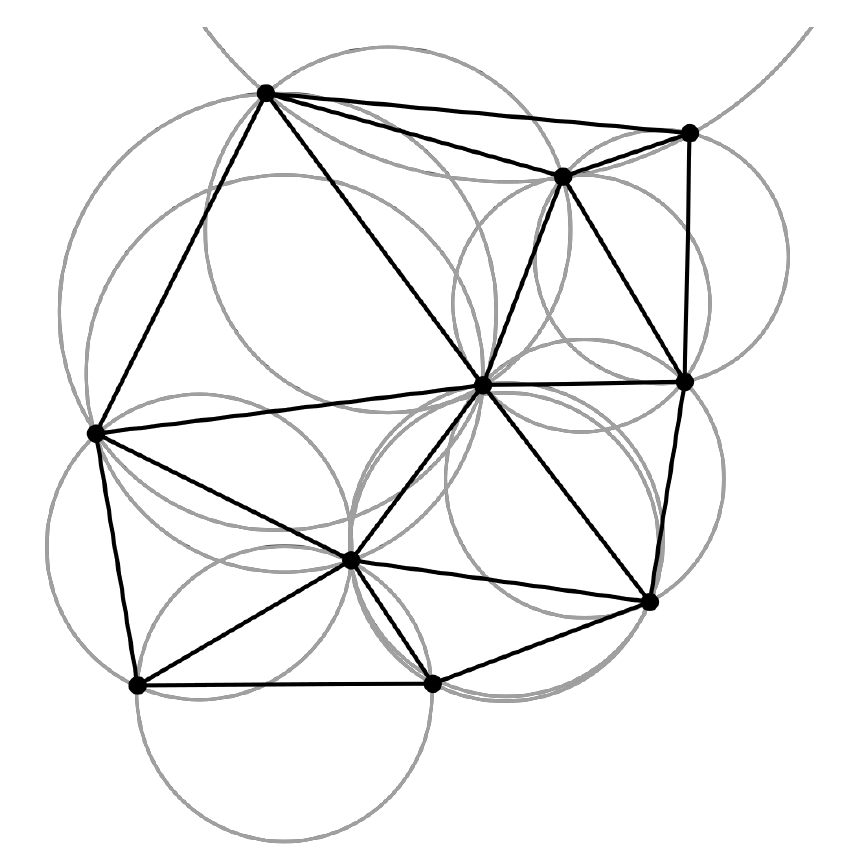
\includegraphics[width=\textwidth]{figs/L07-delaunay-triangulation.png}
            % \caption{Caption}
            % \label{fig:my_label}
        \end{figure}
    \end{columns}
\end{frame}

\begin{frame}{Delaunay Triangulation Properties}
\begin{itemize}
    \item The Delaunay triangulation is a triangulation which is equivalent to the
nerve of the cells in a Voronoi diagram,
    \item it is the triangulation of the convex hull of the points in the diagram in
which every circumcircle of a triangle is an empty circle
an edge is illegal if we can locally increase the smallest angle by flipping
that edge.
    \item A Delaunay triangulation is unique iff the circumcircle of every triangle
contains exactly three points on its circumference: the vertices of the
triangle.
    \item For instance, the Delaunay diagram of the four vertices of a square is a
square, and can be converted into a triangulation in two different ways
\end{itemize}
    
\end{frame}

\begin{frame}{Computing of The Delaunay Triangulation}
    \begin{columns}
        \column{0.7\textwidth}
        It turns out that it is not necessary to compute the angles to check whether a given edge is legal. Instead, we can use the simple criterion
stated in the next lemma. The correctness of this criterion follows from Thales's Theorem
\begin{block}{}
         Let edge $\overline{p_i p_j}$ be incident to triangles $p_i p_j p_k$ and $p_i p_j p_l$
, and let $C$ be the circle through $p_i$, $p_j$, and $p_k$. 
The edge $\overline{p_i p_j}$ is illegal if and only if the point $p_l$
lies in the interior of $C$. Furthermore, if the points $p_i$, $p_j$, $p_k$, $p_l$ form
a convex quadrilateral and do not lie on a common circle, then exactly one of
$\overline{p_i p_j}$ and $\overline{p_k p_l}$ is an illegal edge.
\end{block}
        \column{0.3\textwidth}
        \begin{figure}
            \centering
            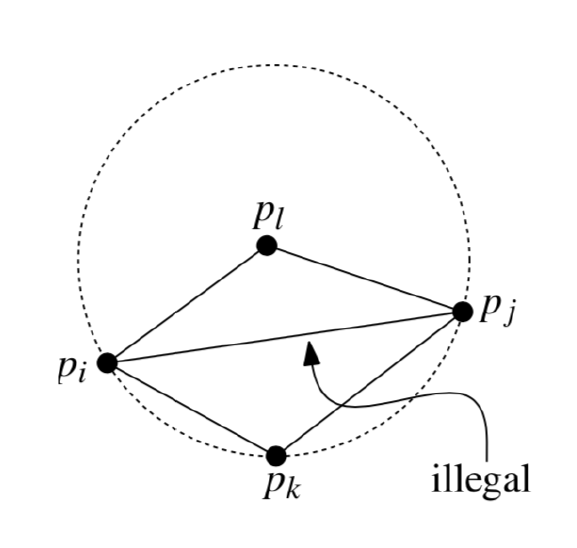
\includegraphics[width=\textwidth]{figs/L07-delaunay-triangulation-illegal.png}
            % \caption{Caption}
            % \label{fig:my_label}
        \end{figure}
    \end{columns}
\end{frame}

\begin{frame}{Computing the Delaunay Triangulation}

We define a legal triangulation to be a triangulation that does not contain
any illegal edge. From the observation above it follows that any angle-optimal
triangulation is legal. Computing a legal triangulation is quite simple, once we
are given an initial triangulation. We simply flip illegal edges until all edges are
legal.

\begin{algorithm}[H]
\SetAlgoLined
\KwIn{
Some triangulation T of a point set P.
}
\KwOut{
A legal triangulation of P.
}
 \While{T contains an illegal edge $\overline{p_i p_j}$}{
    % (Flip )\;
    \Begin(Flip $\overline{p_i p_j}$){
    Let $p_i p_j p_k$ and $p_i p_j p_l$ be the two triangles adjacent to $\overline{p_i p_j}$\;
    Remove $\overline{p_i p_j}$ from T, and add $\overline{p_k p_l}$ instead.
    }
 }
\Return {T}
%  \caption{How to write algorithms}
\end{algorithm}
\end{frame}

\begin{frame}{Voronoi complexes}
    
\end{frame}
\begin{frame}{Voronoi complexes}
    \begin{columns}
        \column{0.7\textwidth}
        \begin{itemize}
            \item  Voronoi diagram is a partitioning of a plane into regions based on distance
to points in a specific subset of the plane.
            \item
That set of points (called seeds, sites, or generators) is specified beforehand,
and for each seed there is a corresponding region consisting of all points
closer to that seed than to any other.  These regions are called Voronoi cells.
            \item
The Voronoi diagram of a set of points is dual to its Delaunay triangulation   
            
        \end{itemize}


        \column{0.3\textwidth}
        \begin{figure}
            \centering
            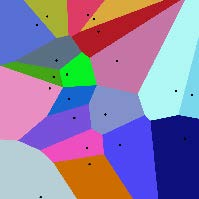
\includegraphics[width=\textwidth]{figs/L07-voronoi.jpg}
            % \caption{Caption}
            % \label{fig:my_label}
        \end{figure}
    \end{columns}
\end{frame}

    % \begin{columns}
    %     \column{0.6\textwidth}
    % \end{columns}
\begin{frame}{The post office problem}
    \begin{figure}
        \centering
        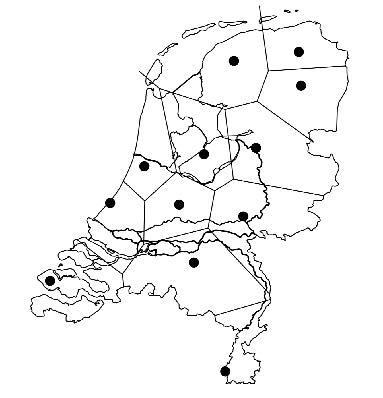
\includegraphics[width=0.5\textwidth]{figs/L07-post-office-problem.jpg}
        
        \caption{The post office problem \cite{DeBerg2008}}
        \label{fig:my_label}
    \end{figure}
    % \begin{columns}
    %     % \column{0.7\textwidth}
    %     % \column{0.3\textwidth}
    % \end{columns}
\end{frame}

% De Berg, M., Cheong, O., Van Kreveld, M., & Overmars, M. (2008). Computational geometry: Algorithms and applications. Computational Geometry: Algorithms and Applications. https://doi.org/10.1007/978-3-540-77974-2
\subsection{Convex hull}

\begin{frame}
\vfill
\centering

\begin{beamercolorbox}[sep=8pt,center,shadow=true,rounded=true]{title}
Convex Hull
\end{beamercolorbox}
\vfill
    
\end{frame}




\begin{frame}{Convex Hull}
    \begin{columns}
        \column{0.6\textwidth}
            Given a discrete set S of points:
            \begin{itemize}
                \item intersection of all convex sets containing S;
                \item minimum convex set containing S
                \item set spanned by all convex combinations of S points
            \end{itemize}
        \column{0.4\textwidth}
        \begin{figure}
            \centering
            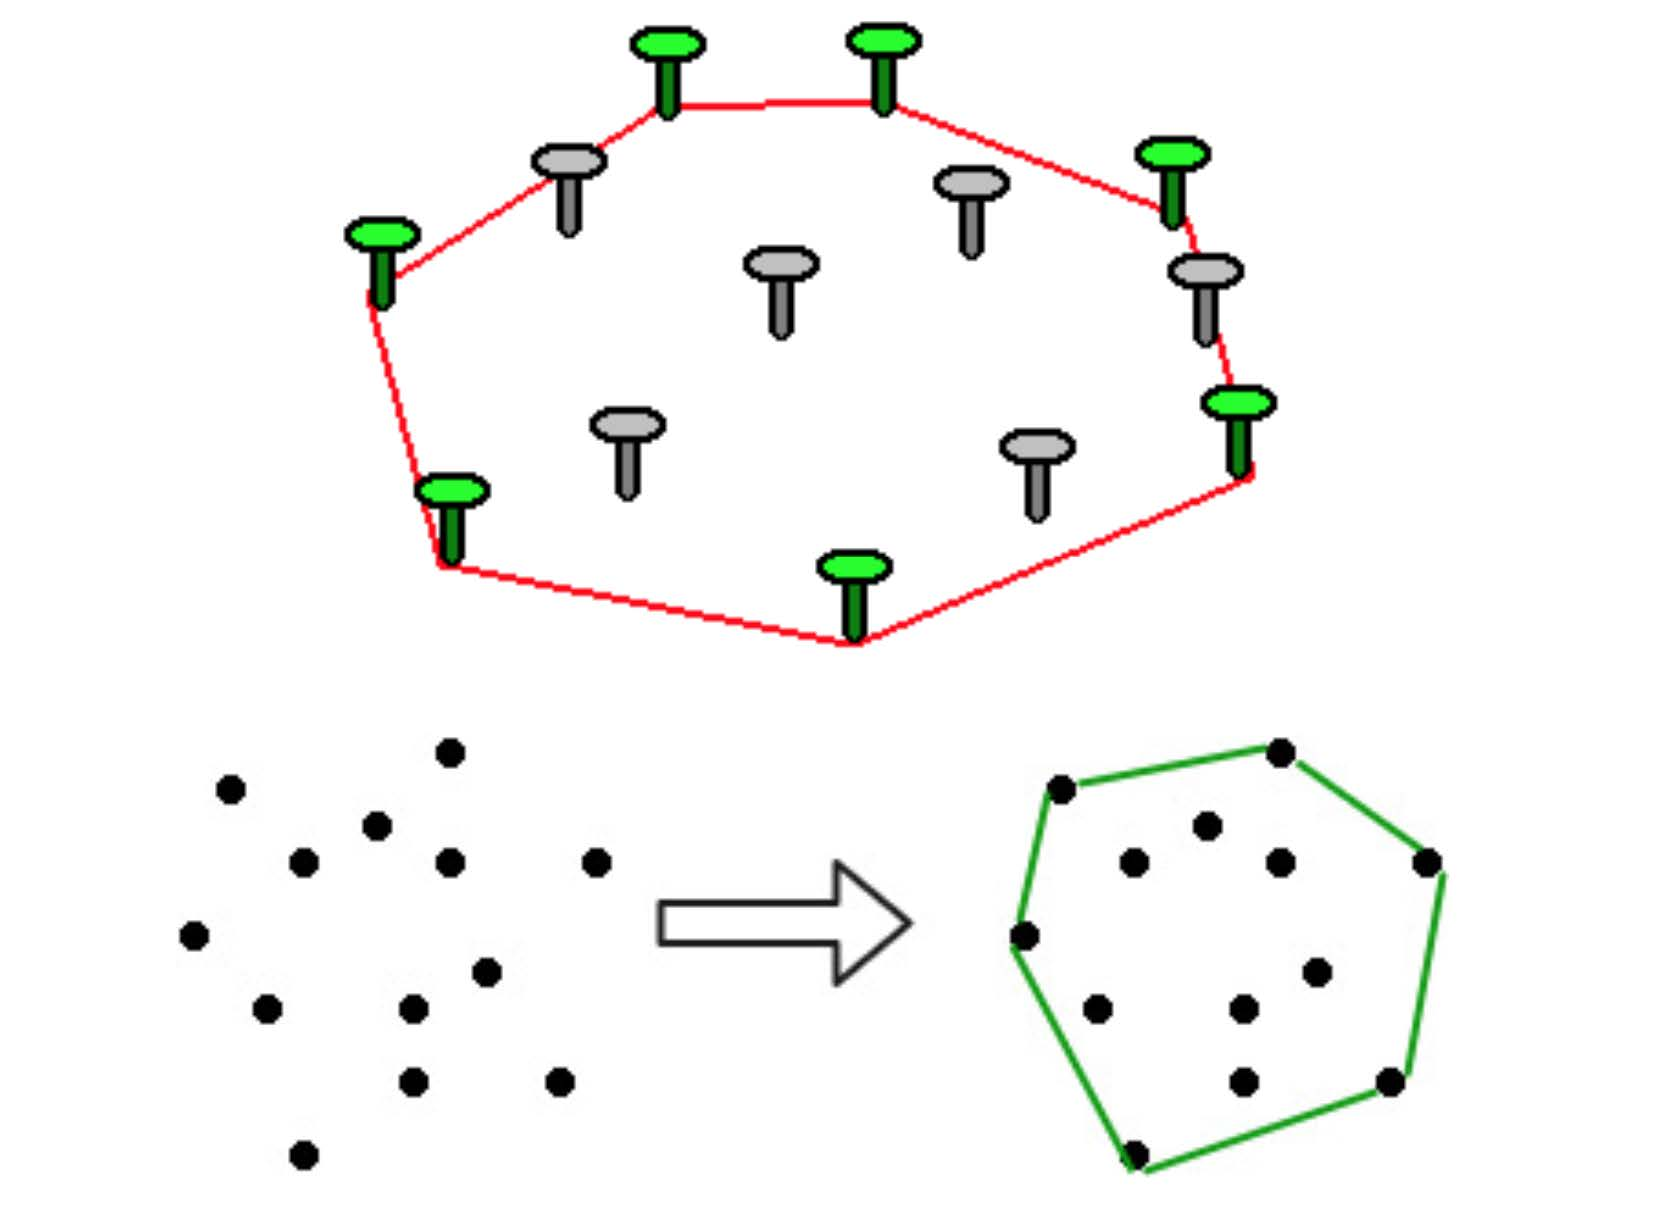
\includegraphics[width=\textwidth]{figs/L14-convex-hull.jpg}
        \end{figure}
    \end{columns}
\end{frame}


\begin{frame}{Jarvis algoritgm\cite{Jarvis1973}}

    Gift Wrap Algorithm (Jarvis March Algorithm) to find Convex Hull. 
    
    O(nh) complexity, where $n = \#S$, and h is the number of points on the
convex hull. Possition is checked by cross product.
        \href{https://en.wikipedia.org/wiki/Gift_wrapping_algorithm}{Demo on Wikipedia}
        \begin{figure}
            \centering
            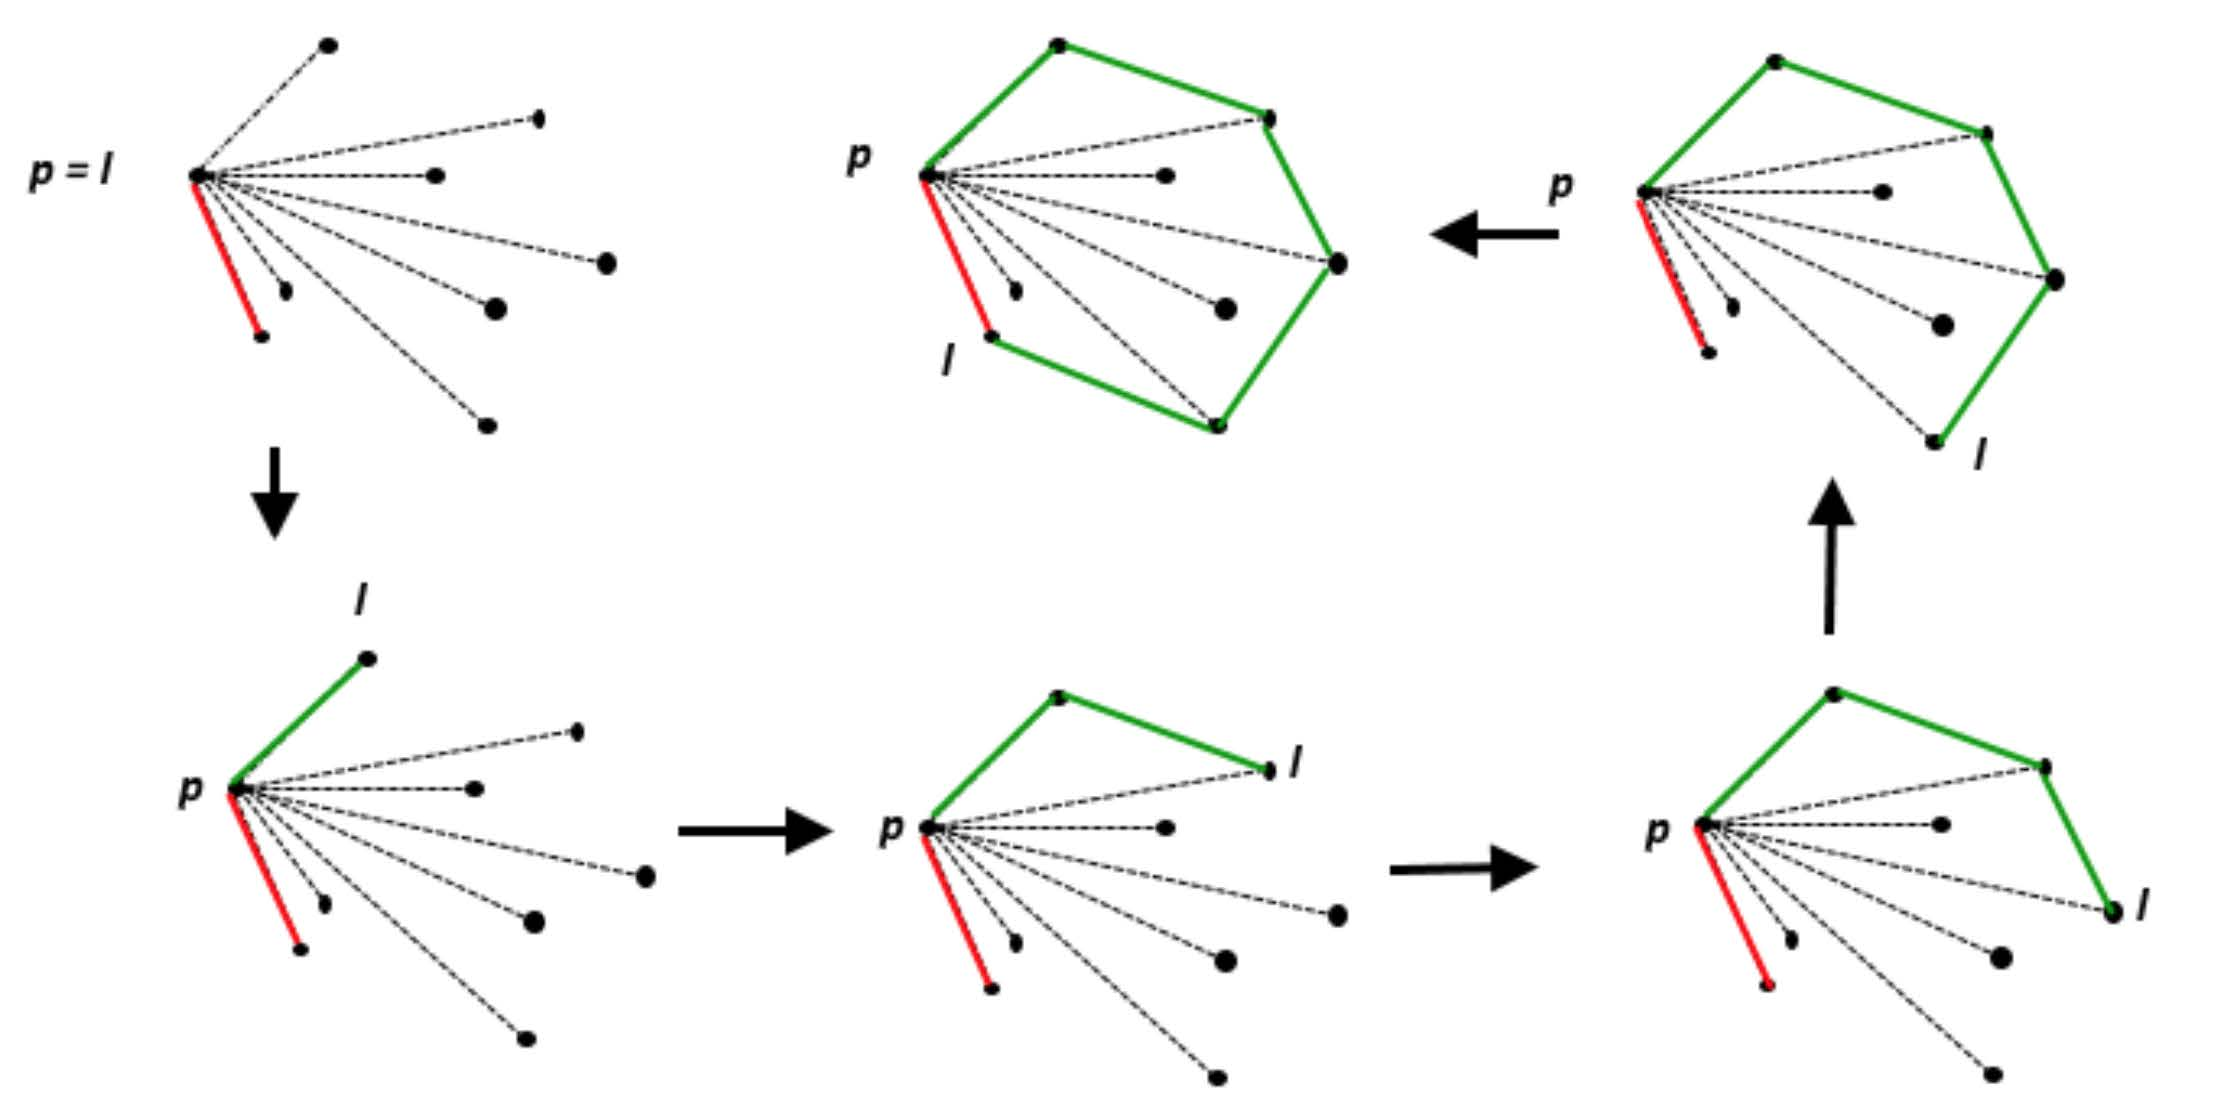
\includegraphics[width=\textwidth]{figs/L14-jarvis-algorithm.jpg}
        \end{figure}
        
    % \begin{columns}
    %     \column{0.7\textwidth}
    %     \column{0.3\textwidth}
    % \end{columns}
\end{frame}

\begin{frame}{Chan's algorithm\cite{Chan1996}}

Chan’s algorithm in the planar case: the algorithm combines an
$O(n \cdot \mathrm{log} ( n))$
algorithm (Graham scan-line, for example) with Jarvis march $O(nh)$, in
order to obtain an optimal $O(n \cdot \mathrm{log}(h))$ time.

\href{https://en.wikipedia.org/wiki/Chan\%27s_algorithm}{Demo on Wikipedia}

    
\end{frame}

\subsection{Alpha shapes}

\begin{frame}{}
        \begin{figure}
            \centering
            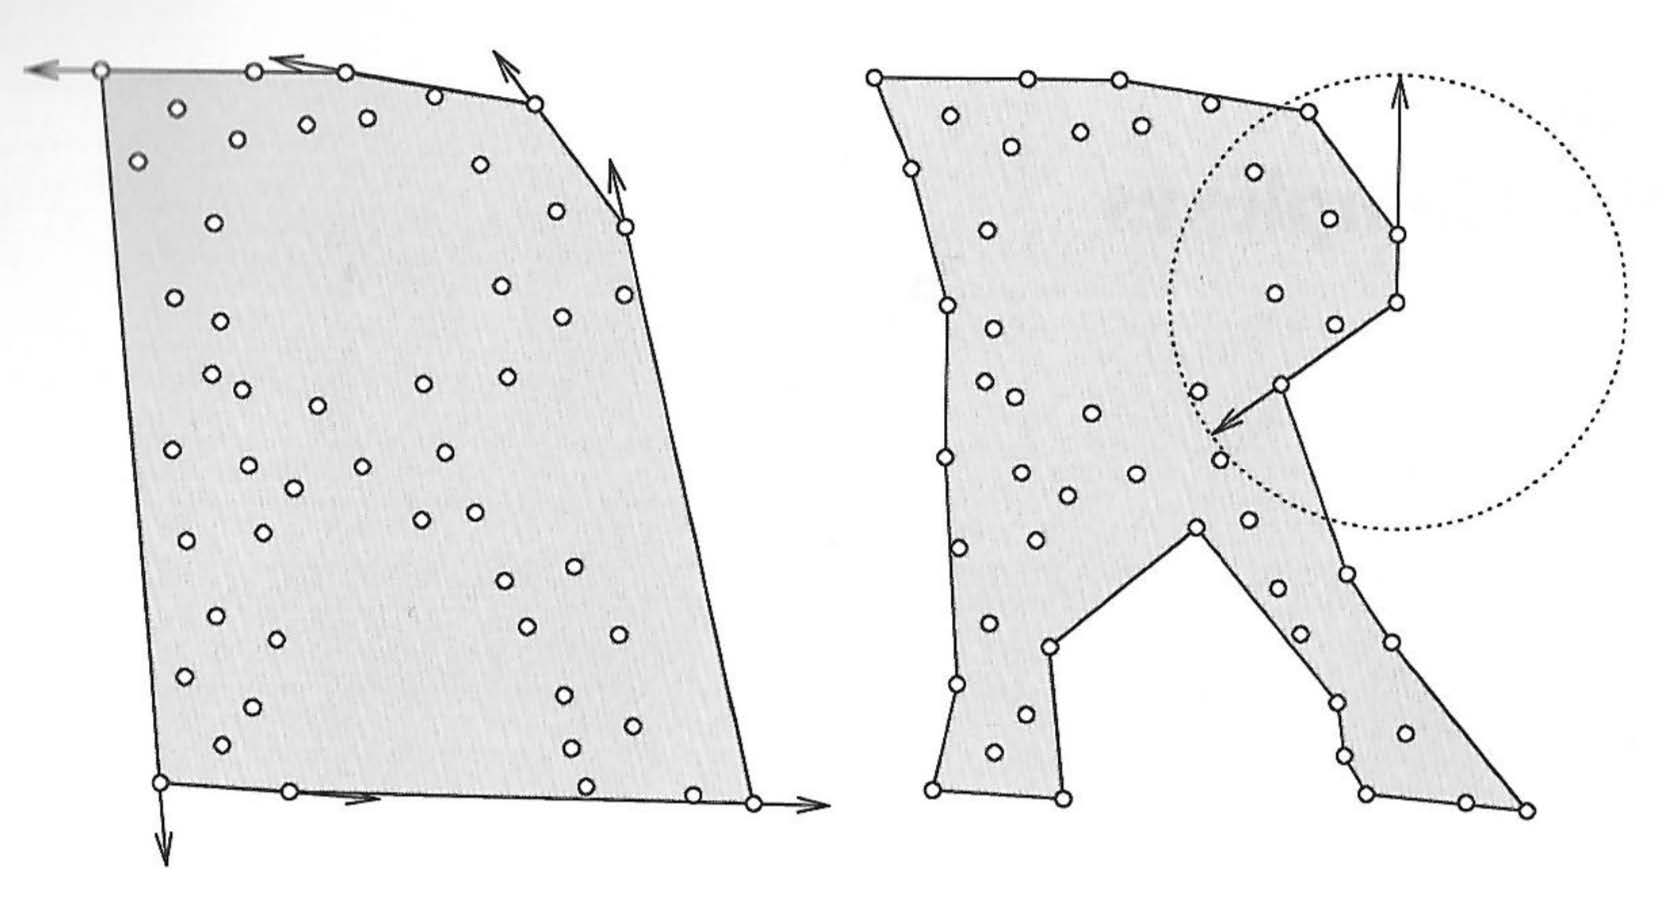
\includegraphics[width=\textwidth]{figs/L14-shape-of-a-set-of-points.jpg}
            \caption{Study the shape of a set of points\cite{edelsbrunner2014short}}
        \end{figure}
\end{frame}



\begin{frame}{Alpha-complexes \cite{Edelsbrunner2010,edelsbrunner1983shape}}
    % \begin{columns}
        % \column{0.7\textwidth}
        \begin{figure}
            \centering
            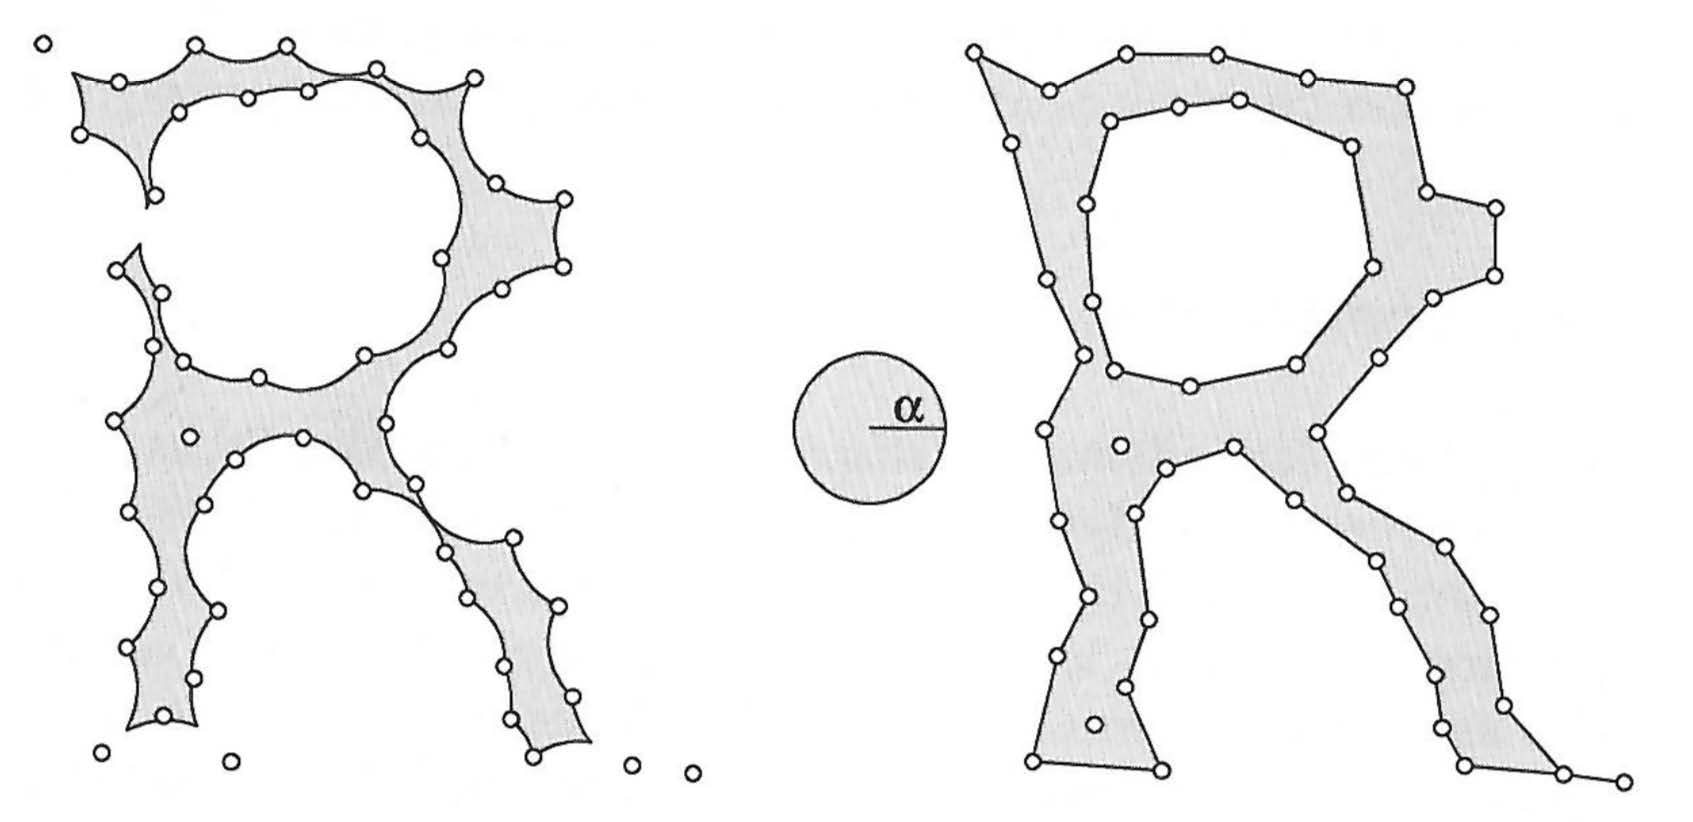
\includegraphics[width=\textwidth]{figs/L14-alpha-hull-alpha-shape.jpg}
            % \caption{Caption}
            % \label{fig:my_label}
        \end{figure}
        % \column{0.3\textwidth}
        
    % \end{columns}
\end{frame}

\begin{frame}{Voronoi decomposition}

    \begin{columns}
        \column{0.5\textwidth}
According to Delaunay triangulation, there is an edge between two points if
their regions intersect in a common edge, and a triangle between three
points if their regions intersect in a common point.
        \column{0.5\textwidth}
        \begin{figure}
            \centering
            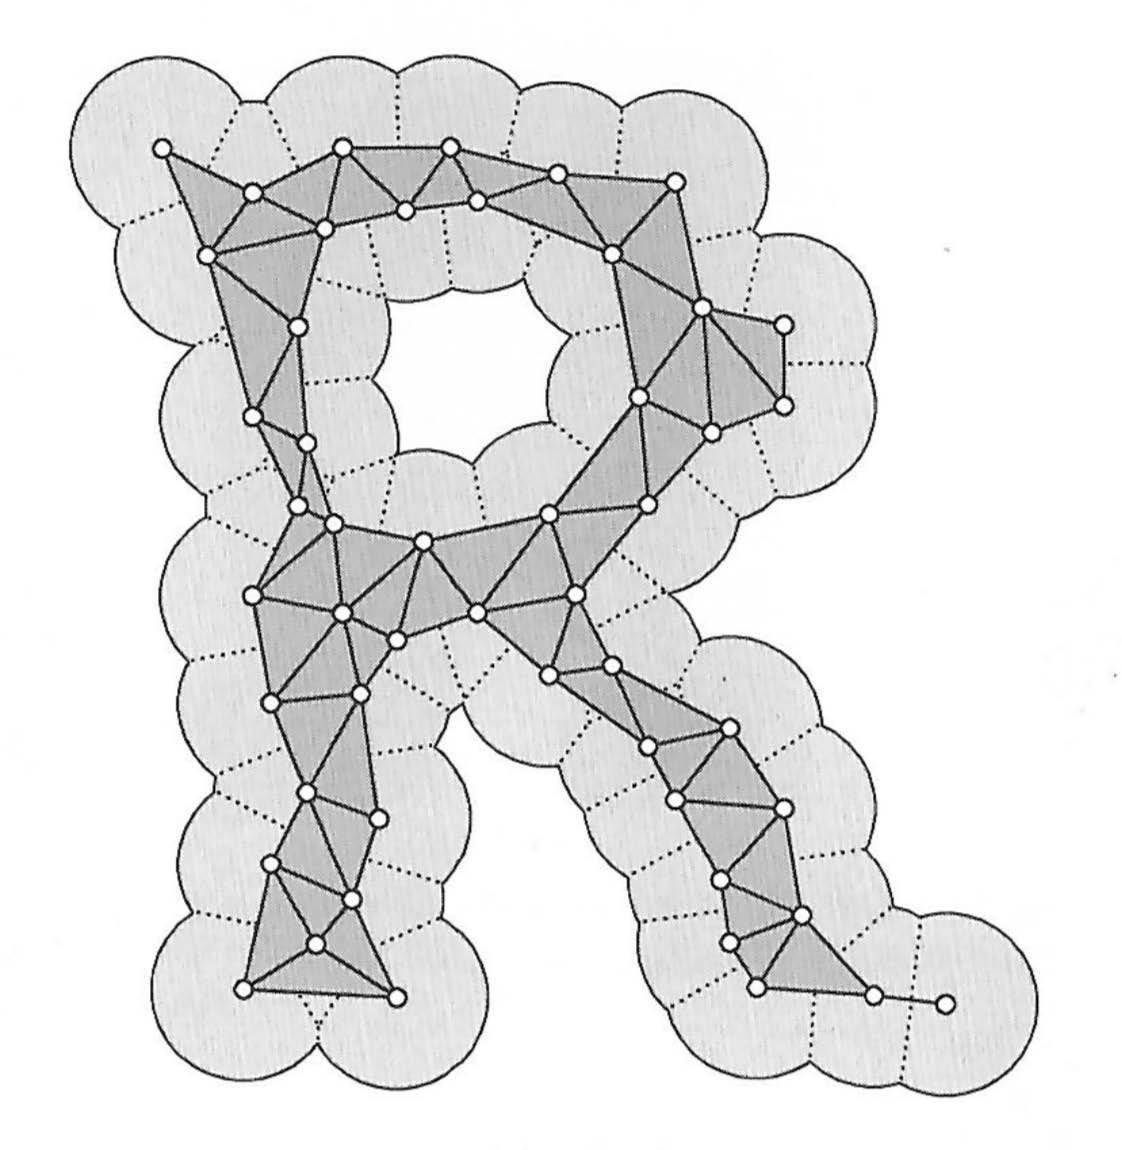
\includegraphics[width=\textwidth]{figs/L14-voronoi.jpg}
        \end{figure}
    \end{columns}
\end{frame}

\begin{frame}{$\alpha$-Complex}
    % \begin{columns}
    %     \column{0.7\textwidth}
    %     \column{0.3\textwidth}
        \begin{figure}
            \centering
            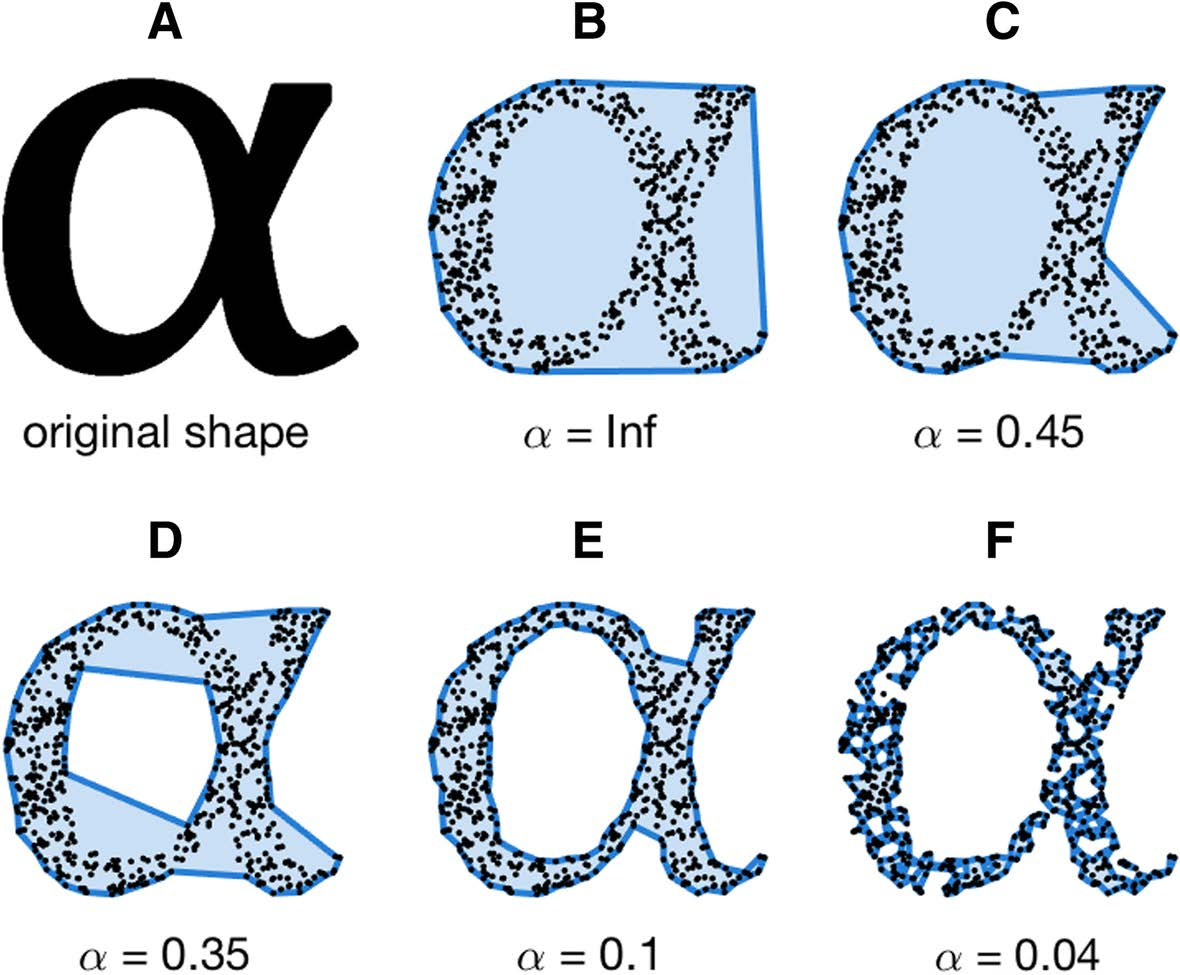
\includegraphics[width=0.65\textwidth]{figs/L14-alpha-complexes-varying-alpha.jpg}
            \caption{$\alpha$-Complexes for varying $\alpha$}
        \end{figure}
    % \end{columns}
\end{frame}

\begin{frame}{$\alpha$-shapes in 3D}
    % \begin{columns}
    %     \column{0.7\textwidth}
    %     \column{0.3\textwidth}
        \begin{figure}
            \centering
            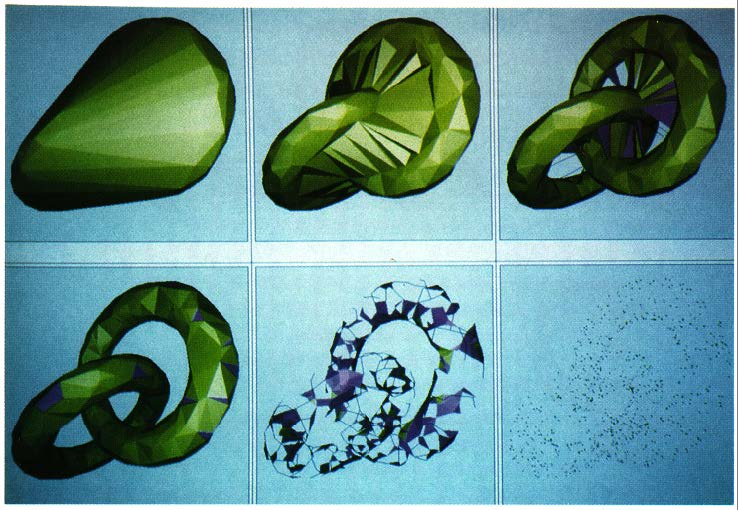
\includegraphics[width=0.9\textwidth]{figs/L19-alpha-shapes-3D-1.jpg}
        \end{figure}
    % \end{columns}
\end{frame}

\begin{frame}{$\alpha$-shapes in 3D}
    % \begin{columns}
    %     \column{0.7\textwidth}
    %     \column{0.3\textwidth}
        \begin{figure}
            \centering
            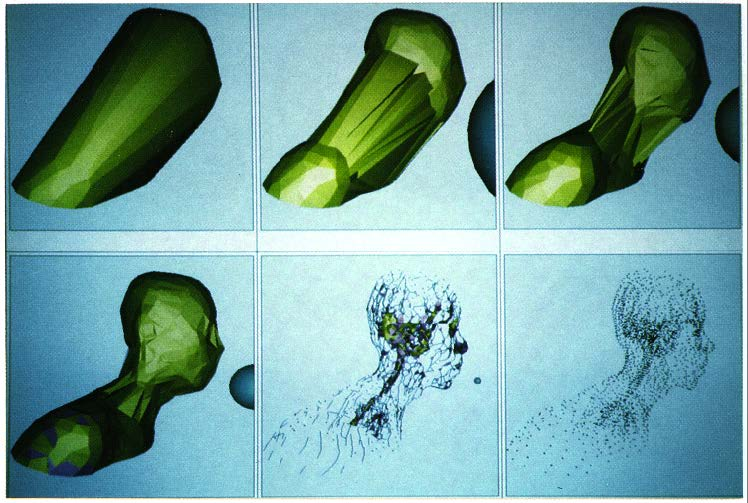
\includegraphics[width=0.9\textwidth]{figs/L19-alpha-shapes-3D-2.jpg}
        \end{figure}
    % \end{columns}
\end{frame}


\subsection{Spatial Hierarchical Domain Trees}
\begin{frame}{Spatial Hierarchical Domain Trees}
    \begin{columns}
        \column{0.5\textwidth}
    Foundations of Multidimensional and
Metric Data Structures provides a
thorough treatment of
multidimensional point data, object
and image-based representations,
intervals and small rectangles, and
high-dimensional datasets

Hanan Samet is the inventor of such
trees (quadtrees and octrees), which
are the foundation of Geographical
databases  \cite{samet2006foundations}
        \column{0.5\textwidth}
        \begin{figure}
            \centering
            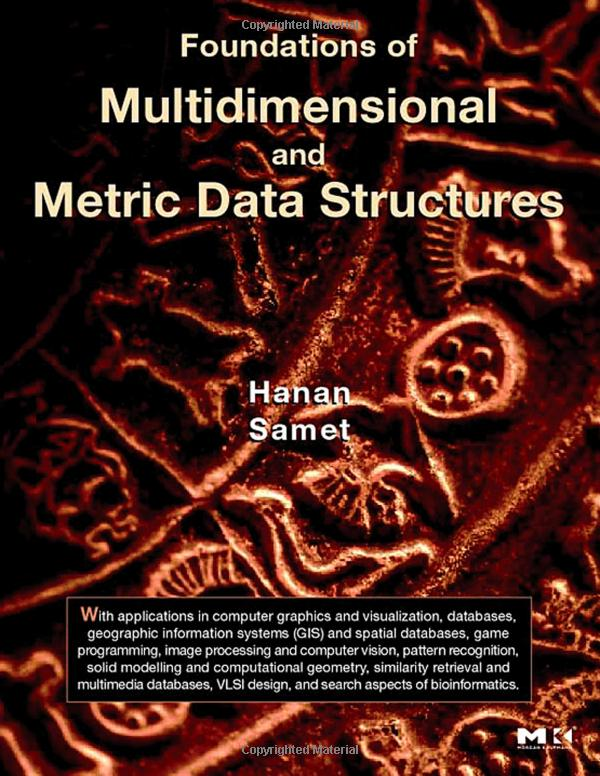
\includegraphics[width=\textwidth]{figs/HananSamet.jpg}
        \end{figure}
    \end{columns}
\end{frame}


\begin{frame}{$2^n$-trees}
$2^n$-trees are ordered trees characterized by the property that each non-leaf
node has exactly $2^n$ son nodes, respectively denoted as first, second, etc.,
and as $2^n$-th son


When n = 2 and n = 3 such trees are called quadtrees and octrees, and are
used to represent hierarchical decompositions of the 2D or 3D space,
respectively

\end{frame}

\begin{frame}{Quadtrees}
\begin{itemize}
    \item a quadtree is a quaternary tree (i.e. each non-leaf node has exactly 4
sons);
    \item the leafs are either white or black nodes (i.e. either empty or full);
    \item the non-leafs are gray nodes (i.e. neither empty nor full);
    \item the maximal depth of the quadtree is related to its resolution.
    \item The number of arcs on the path from the root to a node is called
distance of the node from the root.
    \item Depth of a tree is the maximal distance of its nodes from the root.
    \item The resolution of the quadtree with squared bounding box of size L
and depth m is clearly equal to
\[
r=L/2^m
\]
\end{itemize}
    
\end{frame}


\begin{frame}{Quadtree encoding}
hierarchical decompositive representation using a quadtree, and its actual
encoding as a labeled tree, where black, white and gray nodes represent full
and empty cells, and cells which are neither full nor empty.
The sons of a gray node are clockwise ordered.

\begin{figure}
    \centering
    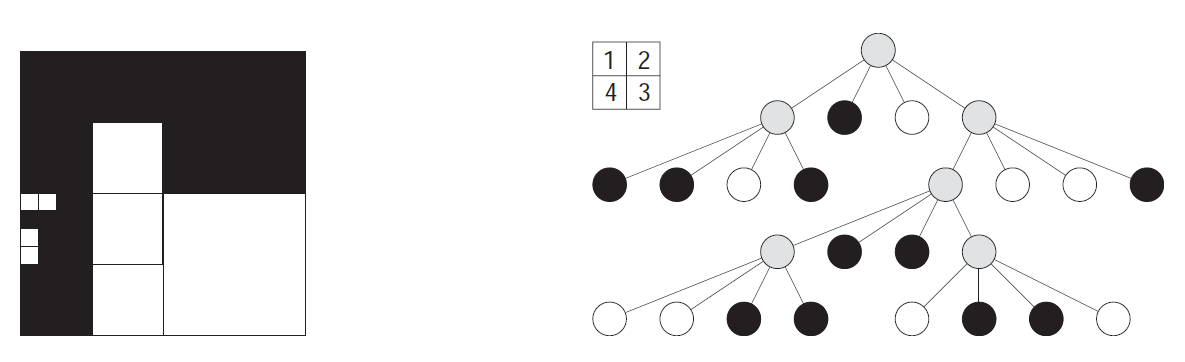
\includegraphics[width=\textwidth]{figs/L17-quad-tree.png}
    \caption{Quadtree encoding scheme: (a) 2D object (b) full cells (black), empty
cells (white) and decomposed cells (gray)}
\end{figure}


    
\end{frame}

\begin{frame}{Octrees}
    \begin{columns}
        \column{0.5\textwidth}
        An octree is a tree data structure in
which each internal node has exactly
eight children. Octrees are most often
used to partition a three-dimensional
space by recursively subdividing it
into eight octants.
        \column{0.5\textwidth}
        \begin{figure}
            \centering
            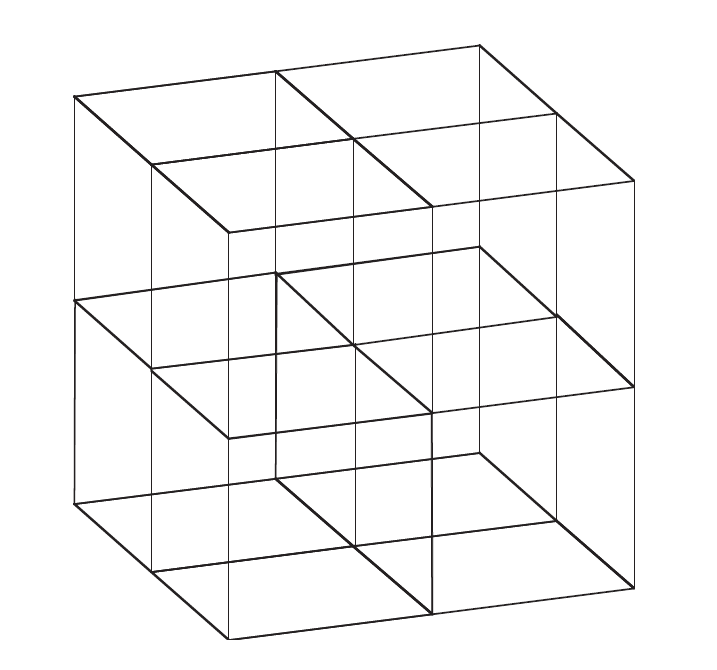
\includegraphics[width=\textwidth]{figs/L17-octree.png}
            \caption{Octree: partition of a 3D cell
into 8 sub-cells generated by three
orthogonal planes}
        \end{figure}
    \end{columns}
\end{frame}


\begin{frame}{Marching Cubes}
\begin{figure}
    \centering
            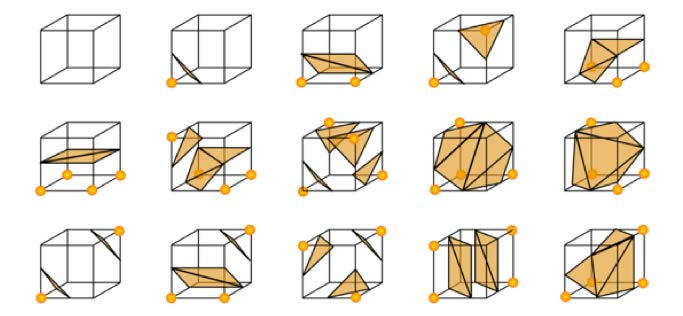
\includegraphics[width=\textwidth]{figs/L16-marching-cubes.jpg}
    \caption{Find the 0-surface (or any iso-surface) of a discrete 3D field \cite{Lorensen1987}}
    \label{fig:my_label}
\end{figure}
    
\end{frame}


\begin{frame}{Surface extraction with LAR}
\begin{figure}
    \centering
            \includegraphics[width=\textwidth]{figs/pao}
    \caption{Liver microstructure\cite{Paoluzzi2016}}
    \label{fig:my_label}
\end{figure}
    
\end{frame}


% \begin{frame}{}
%     \begin{columns}
%         \column{0.7\textwidth}
%         \column{0.3\textwidth}
%         \begin{figure}
%             \centering
%             % \includegraphics[width=\textwidth]{}
%         \end{figure}
%     \end{columns}
% \end{frame}

% \begin{frame}{Frame Title}
%   	Herbert Edelsbrunner and John Harer, [Computational Topology. An Introduction](https://www.amazon.it/Computational-Topology-Introduction-Herbert-Edelsbrunner/dp/0821849255/),  AMS, 2011.

% 3.	Jeremy Kepner and John Gilbert,[Graph Algorithms in the Language of Linear Algebra](epubs.siam.org/doi/book/10.1137/1.9780898719918), 2011.

% 4.	Timothy A. Davis, [Direct Methods for Sparse Linear Systems](http://epubs.siam.org/doi/book/10.1137/1.9780898718881), SIAM, 2006

% 5.	Herbert Edelsbrunner, [Geometry and Topology for Mesh Generation](https://www.amazon.com/Generation-Cambridge-Monographs-Computational-Mathematics/dp/052168207X), Cambridge Monographs on Applied and Computational Mathematics, 2001. \cite{Edelsbrunner2001}
% \end{frame}


% \begin{frame}
% 	\frametitle{Content}
% 	\begin{itemize}
% 		\item Plain GAN
% 			\begin{itemize}
% 				\item[--] General Knowledge
% 				\item[--] Adversarial Loss
% 				\item[--] Problems of the training
% 				\item[--] Examples of Usage 
% 			\end{itemize}
% 		\item Autoencoders
% 			\begin{itemize}
% 				\item[--] Structure
% 				\item[--] Latent-space arithmetic
% 				\item[--] Variational Autoencoder
% 				\item[--] Examples of Usage 
% 			\end{itemize}
% 		\item Condi-GAN
% 			\begin{itemize}
% 				\item[--] General Knowledge
% 				\item[--] Examples of Usage 
% 			\end{itemize}
		
% 	\end{itemize}
% \end{frame}

\endgroup

\begin{frame}{Interval Tree}

    
\end{frame}

\begin{frame}{Delaunay triangulations}

\cite{DeBerg2008}
    
\end{frame}

\subsection{}

% \addtocounter{framenumber}{0}
% \expandafter\def\expandafter\insertshorttitle\expandafter{%
% 	\insertshorttitle \hfill \insertframenumber\,/\,\inserttotalframenumber
% }

% \section[Plain GAN]{Generative Adversarial Networks}

% \begin{frame}
% \frametitle{Supervised vs Unsupervised learning}
% \begin{columns}
% 	\column{.5\textwidth}
% 	\begin{block}{Supervised}
% 		\begin{itemize}
% 			\item Data: (x, y)
% 			\item Goal: Learn a function to map x$\rightarrow$y
% 			\item Examples: Classification, regression, object detection, semantic segmentation
% 		\end{itemize}
% 	\end{block}
% 	\column{.5\textwidth}
% 	\begin{block}{Unsupervised}
% 		\begin{itemize}
% 			\item Data: x
% 			\item Goal: Learn some underlying hidden structure of the data
% 			\item Examples:  Clustering, dimensionality-reduction, feature learning, density estimation, etc
% 		\end{itemize}
% 	\end{block}
% \end{columns}
% \end{frame}

% \begin{frame}
% \frametitle{Discriminative vs Generative models}
% \begin{columns}
% 	\column{.5\textwidth}
% 	\begin{block}{Discriminative}
% 		\begin{itemize}
% 			\item Model differences between classes
% 			\item Decision boundaries between classes
% 			\item Learn conditional probability $p(x|y)$
% 			\item Examples: Logical Regression, SVM, kNN, traditional NN
% 		\end{itemize}
% 	\end{block}
% 	\column{.5\textwidth}
% 	\begin{block}{Generative}
% 		\begin{itemize}
% 			\item Model characteristics of each class
% 			\item Distribution of each class
% 			\item Learn joint probability $p(x,y)$
% 			\item Can generate unseen content!
% 			\item Examples: Naive Bayes, Markov random fields, GANs 
% 		\end{itemize}
% 	\end{block}
% \end{columns}

% \end{frame}

% \begin{frame}
% \frametitle{Generative Adversarial Networks}
% \begin{itemize}
% 	\item Introduced by Goodfellow et al.\footnote{Goodfellow, Ian, et al. "Generative adversarial nets." Advances in neural information processing systems. 2014.}
% 	\item Can be utilized in unsupervised learning tasks
% 	\item Two main parts: generator $G$, and discriminator $D$
% \end{itemize}
% 	\begin{figure}[!ht]
% 	\centering
% 	\includegraphics[width = 0.9\textwidth]{./GAN.png}
% 	\end{figure}
% \end{frame}

% \begin{frame}
% \frametitle{Generator vs Discriminator}
% \begin{columns}
% 	\column{.5\textwidth}
% 	\begin{block}{Generator}
% 		\begin{itemize}
% 			\item Input: $n$-dimensional vector $z$
% 			\item Output: Fake image $x_f$
% 			\item Goal: To produce as realistic output as possible
% 		\end{itemize}
% 	\end{block}
% 	\column{.5\textwidth}
% 	\begin{block}{Discriminator}
% 		\begin{itemize}
%  			\item Input: Real image $x_r$ or Fake image $x_f$
%  			\item Output: Predict label
%  			\item Goal: Distinguish between real and fake images
% 		\end{itemize}
% 	\end{block}
% \end{columns}
% \vspace{1.3cm}
% \centering
% \textbf{Goal}: Nash equilibrium = The discriminator predicts "real" or "fake" with probability 0.5 for any sample.
% \end{frame}

% \begin{frame}
% \frametitle{Adversarial Loss}
% The expected value function of the discriminator:
% \begin{equation} \label{Adversarial_loss}
% V(G,D) = \frac{1}{2}E_{x\sim p_r}[\log D(x)]+\frac{1}{2}E_{z\sim p_z}[\log (1-D(G(z)))],
% \end{equation}

% \begin{equation}
% \min_G(\max_D E(G,D)).
% \end{equation} 
% The best possible discriminator is the one which maximizes:
% \begin{equation}
% E_{x\sim p_r}[\log D(x)]+E_{z\sim p_z}[\log (1-D(G(z)))].
% \end{equation}
% The best possible generator is the one which minimizes:
% \begin{equation}
% E_{z\sim p_z}[\log (1-D(G(z)))].
% \end{equation}
% \end{frame}

% \begin{frame}
% \frametitle{Training Problems - Lack of Convergence}
% 	\begin{itemize}
% 		\item Stems from an unbalance speed of the training
% 		\item The generator is trained faster:
% 		\begin{itemize}
% 			\item The generator becomes superior to the discriminator
% 			\item The generator produces perfect images (from discriminator's point of view)
% 			\item The discriminator is unable to reveal fakes
% 		\end{itemize}
% 		\item The discriminator is trained faster:
% 		\begin{itemize}
% 			\item The discriminator becomes superior to the generator
% 			\item The discriminator flawlessly reveals all fakes
% 			\item The generator does not know what to improve
% 		\end{itemize}
% 		\item Prevention: Heuristic strategies			
% 	\end{itemize}

% \end{frame}

% \begin{frame}
% \frametitle{Training Problems - Mode Collapse}
% 	\begin{itemize}
% 		\item No lever to force the generator to generate different outputs
% 		\item The generator generates only a few different outputs perfectly and omits the rest
% 	\end{itemize}
% 	\begin{figure}[!ht]
% 	\centering
% 	\includegraphics[width = 0.9\textwidth]{./VAEGAN_trans1.png}
% 	\includegraphics[width = 0.9\textwidth]{./VAEGAN_trans2.png}
% \end{figure}
% 	\begin{itemize}
% 		\item Prevention: Wasserstein distance, Conditional GAN
% 	\end{itemize}
% \end{frame}

% \begin{frame}
% \frametitle{Wasserstein Distance}
% \begin{itemize}
% 	\item Replaces standard Adversarial loss
% 	\item Minimum cost of transporting mass
% 	\item Also distance between two different distributions:
% \end{itemize}
% \begin{equation}
% W(p_r, p_g) = \inf_{\gamma\in\Pi(p_r,p_g)}E_{(x,y)\sim\gamma}[||x-y||]
% \end{equation}
% \begin{itemize}
% 	\item Critic replaces discriminator - learn $w$ to find optimal $f_w$
% 	\item Wasserstein loss:
% \begin{equation}
% L(p_r,p_g) = W(p_r, p_g) = \max_{w\in\boldsymbol{W}}E_{x\sim p_r}[f_w(x)]-E_{z\sim p_z}[f_w(G(z))]
% \end{equation}
% \end{itemize}
% \end{frame}

% \begin{frame}
% \frametitle{Applications and examples}
% \begin{itemize}
% 	\item \href{https://github.com/hindupuravinash/the-gan-zoo}{GAN ZOO}
% 	\item \href{https://machinelearningmastery.com/how-to-develop-a-generative-adversarial-network-for-an-mnist-handwritten-digits-from-scratch-in-keras/}{GAN in Keras}, \href{C:/Python36/Scripts/MPV}{Local Example}
% 	\item \href{https://thispersondoesnotexist.com/}{StyleGAN - This person does not exist}
% 	\item \href{https://thisrentaldoesnotexist.com/}{StyleGAN - This rental does not exist}
% 	\item \href{http://thesecatsdonotexist.com/}{StyleGAN - These cats do not exist}
% 	\item \href{https://thiscardoesnotexist.glitch.me/}{StyleGAN - This car does not exist}
% 	\item \href{https://www.thiswaifudoesnotexist.net/}{StyleGAN - This waifu does not exist}
% 	\item \href{http://www.whichfaceisreal.com/index.php}{Which person is real?}
% \end{itemize}

% \end{frame}

% \section[Autoencoders]{Autoencoders}

% \begin{frame}
% \frametitle{Autoencoders}
% \begin{itemize}
% 	\item Unsupervised learning - minimization of reconstruction loss
% 	\item Feed-forward network using "bottleneck" structure
% 	\item Two main parts: Encoder $E$, and Decoder $D$
% \end{itemize}
% 	\begin{figure}[!ht]
% 		\centering
% 		\includegraphics[width = 0.7\textwidth]{./autoencoder.png}
% 	\end{figure}
% \end{frame}

% \begin{frame}
% \frametitle{Encoder, Decoder, and Latent space}
% \begin{columns}
% 	\column{.5\textwidth}
% 	\begin{block}{Encoder}
% 		\begin{itemize}
% 			\item Input: Data $x$
% 			\item Output: latent code $z$
% 			\item Goal: Compress data into a feature vector representation while maintaining important information
% 		\end{itemize}
% 	\end{block}
% 	\column{.5\textwidth}
% 	\begin{block}{Decoder}
% 		\begin{itemize}
% 			\item Input:latent code $z$
% 			\item Output: Decoded data $\hat{x}$
% 			\item Goal: Generate an output map (with the same size as the original input) via upsampling procedure
% 		\end{itemize}
% 	\end{block}
% \end{columns}
% \centering
% \begin{block}{Latent space}
% 	\begin{itemize}
% 		\item No restriction applied to the latent space
% 		\item Over-training leads to dictionarization  
% 	\end{itemize}
% \end{block}
% \end{frame}

% \begin{frame}
% \frametitle{Variational Autoencoder}
% \begin{itemize}
% 	\item Incorporates regularization by explicitly learning a joint distribution over data via forcing the latent space to follow a Gaussian distribution
% 	\item Regularization is added to the loss function
% 	\item Encourages the decoder to learn reconstruct data, while enforce the encoder to follow a Gaussian distribution
% 	\item Pros: Addition of probability allows unseen data generation 
% 	\item Cons: Blurrier samples, harder to train
% \end{itemize}

% \end{frame}

% \begin{frame}{Latent-space arithmetic}
% 	\begin{itemize}
% 		\item Good- trained encoder naturally holds big clustering ability across image attributes despite the lack
% 		of any additional information about them
% 		\item Occurs despite the unsupervised manner of the training and any additional constraints on the latent space
% 		\item Phenomenon occurs with VAE, GAN, VAEGAN, etc.
% 		\item Encoding and Decoding is highly non-linear process, however, some sort of linearity is preserved 
% 	\end{itemize}
% \end{frame}

% \begin{frame}
% \frametitle{Latent-space arithmetic - Example 1}
% \begin{itemize}
% 	\item \href{C:/Python36/Scripts/MPV}{Local example}
% \end{itemize}
% \begin{figure}[!ht]
% 	\centering
% 	\includegraphics[width = 0.9\textwidth]{./latent_geometric.png}
% \end{figure}
% \end{frame}

% \begin{frame}
% \frametitle{Latent-space arithmetic - Example 2}
% \begin{figure}[!ht]
% 	\centering
% 	\includegraphics[width = 0.9\textwidth]{./latent_geometric2.png}
% \end{figure}
% \end{frame}

% \begin{frame}
% \frametitle{AE-GAN}
% \begin{figure}[!ht]
% 	\centering
% 	\includegraphics[width = 0.9\textwidth]{./VAEGAN.png}
% \end{figure}

% \end{frame}

% \begin{frame}
% \frametitle{Application and examples}
% \begin{itemize}
% 	\item \href{D:/Python_scripts/FileGenerator/data/outputs/images}{VAE - document background generation}
% 	\item \href{D:/Dropbox/MPV/Sencor.png}{VAE - Logo detection}
% 	\item \href{D:/Python_scripts/Naki/data_results}{U-Net - Semantic segmentation of historical documents}
% 	\item \href{https://www.kaggle.com/summitkwan/tl-gan-demo}{TL-GAN - Latent-space arithmetic}
% \end{itemize}
% \end{frame}


% \section[Condi-GAN]{}

% \begin{frame}
% \frametitle{Conditional GAN}
% \begin{itemize}
% 	\item Additional condition on generated images
% 	\item Labels act as an extension to the latent space $z$	
% \end{itemize}
% 	\begin{figure}[!ht]
% 	\centering
% 	\includegraphics[width = 0.4\textwidth]{./CondiGan.png}
% 	\end{figure}
% \end{frame}

% \begin{frame}
% \frametitle{Loss Function}
% Standard Adversarial loss:
% \begin{equation}
% V(G,D) = \frac{1}{2}E_{x\sim p_r}[\log D(x)]+\frac{1}{2}E_{z\sim p_z}[\log (1-D(G(z)))].
% \end{equation}
% cGAN loss:
% \begin{equation}
% V(G,D) = \frac{1}{2}E_{x\sim p_r}[\log D(x|y)]+\frac{1}{2}E_{z\sim p_z}[\log (1-D(G(z|y)))].
% \end{equation}
% \end{frame}

% \begin{frame}
% \frametitle{Application and examples}
% \begin{itemize}
% 	\item \href{https://make.girls.moe/}{Anime Girl generation}
% 	\item \href{D:/Python_scripts/pytorch-CycleGAN-and-pix2pix-master/results/feret_sketch_my/test_latest/index.html}{Image-to-sketch translation}
% 	\item \href{http://gandissect.res.ibm.com/ganpaint.html?project=churchoutdoor&layer=layer4}{New-environment generation}
% 	\item Face aging
% 	\item New-pose generation
% 	\item Image inpainting 
% \end{itemize}
% \end{frame}



% \setbeamertemplate{headline}{}

% \section[]{}
% \begin{frame}
% 	\begin{center}
% 		\Huge{Thank you for your attention!} \\
% 		\bigskip
% 		\Huge{Questions?}
% 	\end{center}
% \end{frame}


\begin{frame}[t,allowframebreaks]
\frametitle{References}
\bibliographystyle{alpha}
\bibliography{references.bib, references2.bib}
\end{frame}


\end{document}


%\begin{frame}
%	\frametitle{Klasifikace}
%	\begin{itemize}
%		\item Rozpoznávání ( klasifikace, angl. Pattern recognition ) – zařazování předmětů do tříd
%		\item Klasifikátor nerozeznává objekty, nýbrž jejich obrazy (popisy)
%		\item PŘÍZNAKOVÉ ROZPOZNÁVÁNÍ
%		\item STRUKTURÁLNÍ (SYNTAKTICKÉ) ROZPOZNÁVÁNÍ
%	\end{itemize}
%	\begin{figure}[!ht]
%		\centering
%		\includegraphics[width = 0.9\textwidth]{./klasifikace.png}
%	\end{figure}
%\end{frame}
